\documentclass[a4paper,12pt]{article}

\textwidth 17cm \textheight 25cm \evensidemargin 0cm
\oddsidemargin 0cm \topmargin -2cm
\parindent 0pt
%\parskip \bigskipamount

\usepackage{graphicx}
\usepackage[dutch]{babel}
\usepackage{amssymb,amsthm,amsmath}
%\usepackage{dot2texi}
\usepackage[utf8]{inputenc}
\usepackage{nopageno}
\usepackage{pdfpages}
\usepackage{enumerate}
\usepackage{caption}
\usepackage{wrapfig}
\usepackage{pgf,tikz,pgfplots}
\pgfplotsset{compat=1.15}
\usepackage{color}
\usetikzlibrary{arrows}
\usetikzlibrary{patterns}
\usepackage{fancyhdr}
\pagestyle{fancy}
\usepackage[version=3]{mhchem}
\usepackage{multicol}
\usepackage{fix-cm}
\usepackage{setspace}
\usepackage{mhchem}
\usepackage{xhfill}
\usepackage{parskip}
\usepackage{cancel}
\usepackage{mdframed}
\usepackage{url}
\usepackage{mathtools}
\usepackage{changepage}

\newcommand{\todo}[1]{{\color{red} TODO: #1}}

\newcommand{\degree}{\ensuremath{^\circ}}
\newcommand\rad{\qopname\relax o{\mathrm{rad}}}

\newcommand\ggd{\qopname\relax o{\mathrm{ggd}}}

\pgfmathdeclarefunction{gauss}{2}{%
  \pgfmathparse{1/(#2*sqrt(2*pi))*exp(-((x-#1)^2)/(2*#2^2))}%
}

\def\LRA{\Leftrightarrow}

\newcommand{\zrmbox}{\framebox{\phantom{EXE}}\phantom{X}}
\newcommand{\zrm}[1]{\framebox{#1}}

% environment oefening:
% houdt een teller bij die de oefeningen nummert, probeert ook de oefening op één pagina te houden
\newcounter{noefening}
\setcounter{noefening}{0}
\newenvironment{oefening}
{
  \stepcounter{noefening}
  \pagebreak[0]
  \begin{minipage}{\textwidth}
  \vspace*{0.7cm}{\large\bf Oefening \arabic{noefening}}
}{%
  \end{minipage}
}

\usepackage{calc}

% vraag
\reversemarginpar
\newcounter{punten}
\setcounter{punten}{0}
\newcounter{nvraag}
\setcounter{nvraag}{1}
\newlength{\puntwidth}
\newlength{\boxwidth}
\newcommand{\vraag}[1]{
\settowidth{\puntwidth}{\Large{#1}}
\setlength{\boxwidth}{1.5cm}
\addtolength{\boxwidth}{-\puntwidth}
{\large\bf Vraag \arabic{nvraag} \addtocounter{nvraag}{1}}\vspace*{-0.5cm}
{\marginpar{\color{lightgray}\fbox{\parbox{1.5cm}{\vspace*{1cm}\hspace*{\boxwidth}{\Large{#1}}}}}
\vspace*{0.5cm}}
\addtocounter{punten}{#1}}

% arulefill
\def\arulefill{\leavevmode{\xrfill[-5pt]{0.3pt}[lightgray]\endgraf}\vspace*{0.2cm}}

% \arules{n}
\newcommand{\arules}[1]{
\color{lightgray}
%\vspace*{0.05cm}
\foreach \n in {1,...,#1}{
  \vspace*{0.75cm}
  \hrule height 0.3pt\hfill
}\color{black}\vspace*{0.2cm}}

% \arule{x}
\newcommand{\arule}[1]{
\color{lightgray}{\raisebox{-0.1cm}{\rule[-0.05cm]{#1}{0.3pt}}}\color{black}
}

% \abox{y}
\newcommand{\abox}[1]{
\fbox{
\begin{minipage}{\textwidth- 4\fboxsep}
\hspace*{\textwidth}\vspace{#1}
\end{minipage}
}
}

\newcommand{\ruitjes}[1]{
\definecolor{cqcqcq}{rgb}{0.85,0.85,0.85}
\hspace*{-2.5cm}
\begin{tikzpicture}[scale=1.04,line cap=round,line join=round,>=triangle 45,x=1.0cm,y=1.0cm]
\draw [color=cqcqcq, xstep=0.5cm, ystep=0.5cm] (0,-#1) grid (20.5,0);
\end{tikzpicture}
}


\newcommand{\assenstelsel}[5][1]{
\definecolor{cqcqcq}{rgb}{0.65,0.65,0.65}
\begin{tikzpicture}[line cap=round,line join=round,>=triangle 45,x=#1cm,y=#1cm]
\draw [color=cqcqcq,dash pattern=on 1pt off 1pt, xstep=1.0cm,ystep=1.0cm] (#2,#4) grid (#3,#5);
\draw[->,color=black] (#2,0) -- (#3,0);
%\draw[shift={(1,0)},color=black] (0pt,2pt) -- (0pt,-2pt) node[below] {\footnotesize $1$};
%\draw[color=black] (#3.25,0.07) node [anchor=south west] {$x$};
\draw[->,color=black] (0,#4) -- (0,#5);
%\draw[shift={(0,1)},color=black] (2pt,0pt) -- (-2pt,0pt) node[left] {\footnotesize $1$};
\draw[color=black] (0.09,#5.25) node [anchor=west] {\phantom{$y$}};
%\draw[color=black] (0pt,-10pt) node[right] {\footnotesize $0$};
\end{tikzpicture}
}

\newcommand{\getallenas}[3][1]{
\definecolor{cqcqcq}{rgb}{0.65,0.65,0.65}
\begin{tikzpicture}[scale=#1,line cap=round,line join=round,>=triangle 45,x=1.0cm,y=1.0cm]
\draw [color=cqcqcq,dash pattern=on 1pt off 1pt, xstep=1.0cm,ystep=1.0cm] (#2,-0.2) grid (#3,0.2);
\draw[->,color=black] (#2.25,0) -- (#3.5,0);
\draw[shift={(0,0)},color=black] (0pt,2pt) -- (0pt,-2pt) node[below] {\footnotesize $0$};
\draw[shift={(1,0)},color=black] (0pt,2pt) -- (0pt,-2pt) node[below] {\footnotesize $1$};
\draw[color=black] (#3.25,0.07) node [anchor=south west] {$\mathbb{R}$};
\end{tikzpicture}
}

\newcommand{\visgraad}[1]{\begin{tabular}{p{0.5cm}|p{#1}}&\\\hline\\\end{tabular}}

\newcommand{\tekenschema}[2]{\begin{tabular}{p{0.5cm}|p{#1}}&\\\hline\\[#2]\end{tabular}}

% schema van Horner
\newcommand{\schemahorner}{
\begin{tabular}{p{0.5cm}|p{7cm}}
&\\[1.5cm]
\hline\\
\end{tabular}}

% geef tabular iets meer ruimte
\setlength{\tabcolsep}{14pt}
\renewcommand{\arraystretch}{1.5}

\newcommand{\toets}[3]{
\thispagestyle{plain}
\vspace*{-2.5cm}
\begin{tikzpicture}[remember picture, overlay]
    \node [shift={(15.25 cm,-1.6cm)}] {%
        \includegraphics[width=1.8cm]{/home/ppareit/kaa1415/logokaavelgem.png}%
    };%
\end{tikzpicture}

\begin{tabular}{|llc|c|}
\hline
\vspace*{-0.5cm}
&&&\\
Naam & \arule{4cm} & {\Large\bf KA AVELGEM} & \\
\vspace*{-0.75cm}
&&&\\
Klas & \arule{4cm} & {\Large\bf 20...-...-...} & \\
\hline
\vspace*{-0.75cm}
&&&\\
Toets & {\bf #2} & {\large\bf #1} & Beoordeling\\
\vspace*{-0.75cm}
&&&\\
Onderwerp & \multicolumn{2}{l|}{\bf #3} &\\
\hline
\end{tabular}
}

\newcommand{\oefeningen}[1]{

\fancyhead[LE, RO]{\vspace{0.5cm} #1}
%\thispagestyle{plain}

{\bf \Large \centering Oefeningen: #1}

}

\raggedbottom

\newcommand\vl{\qopname\relax o{\mathrm{vl}}}

\newcommand\dom{\qopname\relax o{\mathrm{dom}}}
\newcommand\ber{\qopname\relax o{\mathrm{ber}}}

\newcommand\mC{\qopname\relax o{\mathrm{mC}}}
\newcommand\uC{\qopname\relax o{\mathrm{{\mu}C}}}
\newcommand\C{\qopname\relax o{\mathrm{C}}}

\newcommand\W{\qopname\relax o{\mathrm{W}}}
\newcommand\kW{\qopname\relax o{\mathrm{kW}}}
\newcommand\kWh{\qopname\relax o{\mathrm{kWh}}}


\newcommand\V{\qopname\relax o{\mathrm{V}}}
\newcommand\ohm{\qopname\relax o{\mathrm{\Omega}}}
\newcommand\kohm{\qopname\relax o{\mathrm{k\Omega}}}


\newcommand\N{\qopname\relax o{\mathrm{N}}}

\newcommand\Nperkg{\qopname\relax o{\mathrm{N/kg}}}

\newcommand\Nperm{\qopname\relax o{\mathrm{N/m}}}

\newcommand\gpermol{\qopname\relax o{\mathrm{g/mol}}}


\newcommand\kgperm{\qopname\relax o{\mathrm{kg/m}}}
\newcommand\kgperdm{\qopname\relax o{\mathrm{kg/dm}}}
\newcommand\gpercm{\qopname\relax o{\mathrm{g/cm}}}
\newcommand\gperml{\qopname\relax o{\mathrm{g/ml}}}


\newcommand{\mA}{\;\mbox{mA}}
\newcommand{\A}{\;\mbox{A}}
\newcommand{\MA}{\;\mbox{MA}}

\newcommand{\us}{\;\mu\mbox{s}}
\newcommand\s{\qopname\relax o{\mathrm{s}}}

\newcommand\h{\qopname\relax o{\mathrm{h}}}

\newcommand{\kmperh}{\;\mbox{km/h}}
\newcommand{\mpers}{\;\mbox{m/s}}
\newcommand{\kmpermin}{\;\mbox{km/min}}
\newcommand{\kmpers}{\;\mbox{km/s}}

\newcommand{\mph}{\;\mbox{mph}}

\newcommand{\Hz}{\;\mbox{Hz}}

\newcommand\Gm{\qopname\relax o{\mathrm{Gm}}}
\newcommand\Mm{\qopname\relax o{\mathrm{Mm}}}
\newcommand\km{\qopname\relax o{\mathrm{km}}}
\newcommand\hm{\qopname\relax o{\mathrm{hm}}}
\newcommand\dam{\qopname\relax o{\mathrm{dam}}}
\newcommand\m{\qopname\relax o{\mathrm{m}}}
\newcommand\dm{\qopname\relax o{\mathrm{dm}}}
\newcommand\cm{\qopname\relax o{\mathrm{cm}}}
\newcommand\mm{\qopname\relax o{\mathrm{mm}}}
\newcommand\um{\qopname\relax o{\mathrm{{\mu}m}}}
\newcommand\nm{\qopname\relax o{\mathrm{nm}}}


\newcommand\Gg{\qopname\relax o{\mathrm{Gg}}}
\newcommand\Mg{\qopname\relax o{\mathrm{Mg}}}
\newcommand\kg{\qopname\relax o{\mathrm{kg}}}
\newcommand\hg{\qopname\relax o{\mathrm{hg}}}
\renewcommand\dag{\qopname\relax o{\mathrm{dag}}}
\newcommand\g{\qopname\relax o{\mathrm{g}}}
\newcommand\dg{\qopname\relax o{\mathrm{dg}}}
\newcommand\cg{\qopname\relax o{\mathrm{cg}}}
\newcommand\mg{\qopname\relax o{\mathrm{mg}}}
\newcommand\ug{\qopname\relax o{\mathrm{{\mu}g}}}
\renewcommand\ng{\qopname\relax o{\mathrm{ng}}}

\newcommand\ton{\qopname\relax o{\mathrm{ton}}}

\newcommand\Gl{\qopname\relax o{\mathrm{Gl}}}
\newcommand\Ml{\qopname\relax o{\mathrm{Ml}}}
\newcommand\kl{\qopname\relax o{\mathrm{kl}}}
\newcommand\hl{\qopname\relax o{\mathrm{hl}}}
\newcommand\dal{\qopname\relax o{\mathrm{dal}}}
\renewcommand\l{\qopname\relax o{\mathrm{l}}}
\newcommand\dl{\qopname\relax o{\mathrm{dl}}}
\newcommand\cl{\qopname\relax o{\mathrm{cl}}}
\newcommand\ml{\qopname\relax o{\mathrm{ml}}}
\newcommand\ul{\qopname\relax o{\mathrm{{\mu}l}}}
\newcommand\nl{\qopname\relax o{\mathrm{nl}}}

\newcommand\MJ{\qopname\relax o{\mathrm{MJ}}}
\newcommand\kJ{\qopname\relax o{\mathrm{kJ}}}
\newcommand\J{\qopname\relax o{\mathrm{J}}}

\newcommand\T{\qopname\relax o{\mathrm{T}}}
\newcommand\uT{\qopname\relax o{\mathrm{{\mu}T}}}

\newcommand\grC{\qopname\relax o{\mathrm{{\degree}C}}}

\newcommand\K{\qopname\relax o{\mathrm{K}}}
\newcommand\calperK{\qopname\relax o{\mathrm{cal/K}}}

\newcommand\hPa{\qopname\relax o{\mathrm{hPa}}}
\newcommand\Pa{\qopname\relax o{\mathrm{Pa}}}

\newcommand\dB{\qopname\relax o{\mathrm{dB}}}

\newcommand\Var{\qopname\relax o{\mathrm{Var}}}

\newcommand{\EE}[1]{\cdot 10^{#1}}

\onehalfspacing

%\setlength{\headsep}{0cm}

\newenvironment{exlist}[1] %
{ \begin{multicols}{#1}
  \begin{enumerate}[(a)]
    \setlength{\itemsep}{0.5em} }
{ \end{enumerate}
  \end{multicols} }




\begin{document}

\thispagestyle{empty}
\begin{center}
  \begin{mdframed}
  \centering
  \fontsize{40}{50}\selectfont Goniometrische functies
  \end{mdframed}
  \vfill
  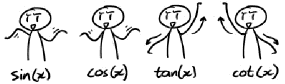
\includegraphics[width=0.7\textwidth]{gon-dance-moves}
  \vfill
\end{center}
\subsection*{Doelstelling}
Je \hfill  {\scriptsize(LP 2006-059, LI 1.6)}
\begin{itemize}
  \item kent de definitie van radiaal, kan het verband leggen tussen graden en radialen en kan de sinus, cosinus en tangens van een reëel getal berekenen
  \item kan de goniometrische getallen van verwante hoeken berekenen
  \item kan de grafiek van de functies $f(x)=\sin x$ , $f(x)=\cos x$ en $f(x)=\tan x$ construeren vanuit de goniometrische cirkel
  \item kan van de functies $f(x)=\sin x$ , $f(x)=\cos x$ en $f(x)=\tan x$ de tabel, het domein, enkele bijzondere waarden, de periodiciteit, het stijgen/dalen en de eventuele extrema bepalen
  \item kan aan de hand van de grafiek het domein, het bereik, de nulwaarden, het tekenverloop, de periodiciteit, het stijgen\&dalen en de extrema bepalen van goniometrische functies  
  \item kan de grafiek opbouwen van de functie $f(x) = a \sin(bx+c)+d$ en kunnen op deze grafiek de betekenis van $a$, $b$, $c$ en $d$ interpreteren
  \item kan goniometrische vergelijkingen van de vorm $\sin x = k$ , $\cos x = k$ en $\tan x = k$ grafisch oplossen
  \item kan vraagstukken/problemen oplossen die aanleiding geven tot een goniometrische vergelijking of functie
\end{itemize}

\pagestyle{empty}
\mbox{}
\newpage
\clearpage
\thispagestyle{empty}
%\mbox{}
{\small \singlespacing \tableofcontents}
\newpage
\clearpage
\pagenumbering{arabic} 

\pagestyle{fancy}
\lhead{}
\rhead{Goniometrische functies}

\onehalfspacing


\section{Hoekeenheden}
Op onze rekenmachine vinden we in \zrm{MODE} 3 soorten hoekeenheden:\\

\textbf{RAD} = radialen

\textbf{DEG} = zestigdelige graden

\textbf{GRA} = honderddelige graden

\subsection{De zestigdelige graad}
Een zestigdelige graad is het 90ste deel van een rechte hoek.\\
\begin{center}
1 rechte hoek = $90\degree$\\
$1\degree = 60'$ (minuten)\\
$1' = 60''$ (seconden)\\
\end{center}
Voor de oorsprong van deze vreemde onderverdeling, in relatie tot ons decimaal talstelsel, moeten we terug naar de Babyloniërs. Voor hen bestond een jaar uit 360 dagen. De kalender was nog lang niet volmaakt, aangezien een totaal van 360 dagen inhield dat om de zoveel jaar extra periodes moesten worden ingelast, de schrikkelmaanden, zodat de kalender gelijk opging met de seizoenen. Uit hun onderzoeken volgde ook de verdeling van de dag in uren, en met behulp van wiskundige berekeningen volgens een zestigtallig stelsel werden de uren opgedeeld in minuten en seconden.
Dit is dezelfde opdeling die wij gebruiken om hoeken te meten!

De zestigdelige graad is nu eenmaal geen zo een handige talstelsel om in te rekenen. Gelukkig hebben wij wiskundigen hier een oplossing voor gevonden. We hebben gewoon nog een nieuwe eenheid ingevoerd, de radiaal!

\pagebreak
\subsection{De radiaal}
De meest natuurlijke hoekeenheid is echter de radiaal. Het woord radiaal is afgeleid van het Latijnse woord ‘radius’, dat straal betekent.

\subsubsection{Definitie}
\begin{minipage}{0.5\textwidth}
De hoekgrootte van een middelpuntshoek waarvan de bijbehorende cirkelboog precies even lang is als de straal van de cirkel, noemen we de {\bf radiaal} ($1 \rad$).
\end{minipage}
\begin{minipage}{0.5\textwidth}
\vspace*{-1cm}
\begin{center}
\definecolor{wqwqwq}{rgb}{0.4,0.4,0.4}
\begin{tikzpicture}[line cap=round,line join=round,>=triangle 45,x=2.0cm,y=2.0cm]
\draw[->,color=black] (-1.5328277784215052,0.) -- (1.6277261422339706,0.);
\foreach \x in {-1.,1.}
\draw[shift={(\x,0)},color=black] (0pt,2pt) -- (0pt,-2pt) node[below] {\footnotesize $\x$};
\draw[->,color=black] (0.,-1.567215720415761) -- (0.,1.3732996361434509);
\foreach \y in {-1.,1.}
\draw[shift={(0,\y)},color=black] (2pt,0pt) -- (-2pt,0pt) node[left] {\footnotesize $\y$};
\draw[color=black] (0pt,-10pt) node[right] {\footnotesize $0$};
\clip(-1.5328277784215052,-1.567215720415761) rectangle (1.6277261422339706,1.3732996361434509);
\draw [shift={(0.,0.)},fill=black,fill opacity=0.1] (0,0) -- (0.:0.30005258740400087) arc (0.:57.29577951308232:0.30005258740400087) -- cycle;
\draw(0.,0.) circle (1);
\draw [shift={(0.,0.)},line width=2.pt]  plot[domain=0.:1.,variable=\t]({1.*1.*cos(\t r)+0.*1.*sin(\t r)},{0.*1.*cos(\t r)+1.*1.*sin(\t r)});
\draw (0.3,0.33) node[anchor=north west] {$1 \rad$};
\draw [line width=1.6pt] (0.,0.)-- (1.,0.);
\draw [line width=1.2pt,dotted] (0.,0.)-- (0.5403023058681398,0.8414709848078965);
\begin{scriptsize}
\draw [fill=wqwqwq] (1.,0.) circle (1.5pt);
\draw [fill=wqwqwq] (0.5403023058681398,0.8414709848078965) circle (1.5pt);
\draw [fill=wqwqwq] (0.,0.) circle (1.5pt);
\end{scriptsize}
\end{tikzpicture}
\end{center}
\end{minipage}

\subsubsection{Verband tussen radialen en zestigdelige graden}

Het getal $\pi$ wordt gedefinieerd als het getal dat we krijgen wanneer we de omtrek van een cirkel delen door de diameter van die cirkel. Dus als we een cirkel met diameter 1 nemen, dan heeft de omtrek lengte $\pi$. Onze éénheidscirkel heeft straal $r=1$, dus de diameter is $2$ en dus de omtrek van de éénheidscirkel is $2\pi$. Hieruit volgt dus dat er voor een volle hoek van $360\degree$ geldt:
\begin{mdframed}
$$360\degree = 2\pi \rad$$
\end{mdframed}


Een rechte hoek meet dus $\frac{\pi}{2}$ en een gestrekte hoek meet dus $\pi \rad$. Omdat de omtrek van de goniometrische cirkel $2\pi$ is, is de maat van de nulhoek niet ondubbelzinnig bepaald. De nulhoek meet zowel $0 \rad$ als $2\pi \rad$. We moeten dus de maatgetallen in radialen slechts op een geheel veelvoud van $2\pi$ na bepalen:

\begin{mdframed}
$$\forall \alpha \in \mathbb{R} : \alpha \rad = (\alpha + k2\pi) \rad (k\in \mathbb{Z})$$
\end{mdframed}

\subsubsection{Graden omzetten in radialen}
We kunnen nu de omzetting berekenen met behulp van het volgende verband:
\begin{alignat*}{2}
     &&360\degree &= 2\pi \rad\\
\LRA &&180\degree &= \pi \rad\\
\LRA &&  1\degree &= \frac{\pi}{180} \rad\\[1em]
\LRA &&  x\degree &= x\cdot\frac{\pi}{180\degree} \rad
\end{alignat*}

\begin{oefening}
Vul de tabel aan met radialen.
\begin{center}
  \begin{tabular}{c|c|c|c|c|c|c|c|c|c}
    $0\degree$ & $30\degree$ & $45\degree$ & $60\degree$ &$90\degree$ &$120\degree$ &$135\degree$ &$150\degree$ &$180\degree$ & $270\degree$ \\
    \hline
   &&&$\frac{1}{3}\pi$&&&&&&\\
  \end{tabular}
\end{center}
\end{oefening}

\subsubsection{Van graden, minuten en seconden naar radialen}

We zetten met het \zrm{ZRM} $309\degree 23' 50''$ om in radialen:

$$309\degree 23' 50''=309\degree 23' 50''\cdot \dfrac{\pi}{180\degree}=5.4\rad$$

\subsubsection{Radialen omzetten in graden}
We kunnen de omzetting berekenen met behulp van het volgende verband:
\begin{alignat*}{2}
     &&2\pi\rad &=360\degree\\
\LRA &&\pi \rad &=180\degree\\
\LRA &&  1 \rad &= \frac{180\degree}{\pi}\\[1em]
\LRA &&  x \rad &= x\cdot\frac{180\degree}{\pi}
\end{alignat*}

\paragraph{Voorbeeld:}
$$5.4 \rad=5.4\cdot\dfrac{180\degree}{\pi}=309\degree 23' 50''$$

\begin{oefening} Zet om in radialen
\begin{multicols}{2}
\begin{enumerate}[(a)]
  \itemsep1em
  \item $75\degree=$\arulefill
  \item $215\degree=$\arulefill
  \item $-75\degree=$\arulefill
  \item $15\degree=$\arulefill
  \item $2.17\degree=$\arulefill
  \item $-35\degree25'47"=$\arulefill
  \item $106\degree20'=$\arulefill
  \item $316\degree2'25"=$\arulefill
\end{enumerate}
\end{multicols}
\end{oefening}

\begin{oefening} Zet om in zestigdelige graden, minuten en seconden
\begin{multicols}{2}
\begin{enumerate}[(a)]
  \item $\pi \rad=$\arulefill
  \item $\dfrac{2\pi}{3} \rad=$\arulefill
  \item $\dfrac{5\pi}{4} \rad=$\arulefill
  \item $\dfrac{-3\pi}{2} \rad=$\arulefill
  \item $\dfrac{\pi}{15} \rad=$\arulefill
  \item $\dfrac{-2\pi}{5} \rad=$\arulefill
  \item $2.86 \rad=$\arulefill
  \item $6 \rad=$\arulefill
  \item $0.456 \rad=$\arulefill
  \item $-0.75 \rad=$\arulefill 
\end{enumerate}
\end{multicols}
\end{oefening}

\subsubsection{Opmerking}
In het vervolg zullen we de eenheid '$\rad$' niet meer vermelden. Wanneer we bv. spreken over een hoek  $\dfrac{2\pi}{3}$, bedoelen we dus steeds  $\dfrac{2\pi}{3} \rad$. Vanaf nu stappen we ook af van de zestigdelige graden en zullen we alles meten in radialen.

\newpage
\section{De goniometrische functies}
\subsection{De sinusfunctie}
\subsubsection{Tabel}
Vul onderstaande tabel aan. De hoek $x$ is uitgedrukt in radialen. Rond af op 2 decimalen.

\begin{adjustwidth}{-2.5cm}{-2.5cm}
\begin{center}
  \begin{tabular}{c|c|c|c|c|c|c|c|c|c|c|c|c}
    $x$ & -1 & 0 & 1 &  $\frac{\pi}{2}$ & 2 & 3 & $\pi$ & 4 & $\frac{3\pi}{2}$ & 5 & 6 & $2\pi$\\
    \hline
   $\sin x$ &\hspace*{0.5cm}&\hspace*{0.5cm}&\hspace*{0.5cm}&\hspace*{0.5cm}&\hspace*{0.5cm}&\hspace*{0.5cm}&\hspace*{0.5cm}&\hspace*{0.5cm}&\hspace*{0.5cm}&\hspace*{0.5cm}&\hspace*{0.5cm}&\hspace*{0.5cm}
  \end{tabular}
\end{center}
\end{adjustwidth}

\subsubsection{Grafiek} 
\begin{center}
\definecolor{cqcqcq}{rgb}{0.75,0.75,0.75}
\definecolor{lightgray}{rgb}{0.95,0.95,0.95}
\begin{tikzpicture}[yscale=1.3,line cap=round,line join=round,>=triangle 45,x=1.0cm,y=1.0cm]
\draw [color=cqcqcq,dash pattern=on 1pt off 1pt, xstep=1.0cm,ystep=1.0cm] (-5.21,-1.47) grid (8.61,1.35);
\draw[->,color=black] (-5.21,0) -- (8.61,0);
\foreach \x in {-5,-4,-3,-2,-1,1,2,3,4,5,6,7,8}
\draw[shift={(\x,0)},color=black] (0pt,2pt) -- (0pt,-2pt) node[below] {\footnotesize $\x$};
\draw[->,color=black] (0,-1.47) -- (0,1.35);
\foreach \y in {-1,1}
\draw[shift={(0,\y)},color=black] (2pt,0pt) -- (-2pt,0pt) node[left] {\footnotesize $\y$};
\draw[color=black] (0pt,-10pt) node[right] {\footnotesize $0$};
\clip(-5.21,-1.47) rectangle (8.61,1.35);
\draw[color=lightgray, line width=1.2pt, smooth,samples=100,domain=-5.211247613943133:8.61062736834769] plot(\x,{sin(((\x))*180/pi)});
\end{tikzpicture}
\end{center}

\subsubsection{Kenmerken van de sinusfunctie}
\begin{oefening}
Vul de kenmerken aan van de sinusfunctie.
\begin{enumerate}[(a)]
  \item $\dom \sin=\arule{3cm}$ en $\ber \sin=\arule{3cm}$
%  \item Periode\\ We merken op dat de sinusfunctie zichzelf steeds herhaalt. We zeggen dat de sinusfunctie periodiek is. De periode van de sinusfunctie is de kleinste afstand waarbij de functie zichzelf herhaalt. Duid deze afstand aan op de grafiek. Voor de sinusfunctie is dit $P=$....................
  \item Nulwaarden:
  \arules{3}
  \item Tekenverloop: 
  \begin{center}
    \visgraad{10cm}
  \end{center}
  \item Stijgen\&dalen en extreme waarden:
  \begin{center}
    \visgraad{10cm}
  \end{center}
\end{enumerate}
\end{oefening}

\subsection{De cosinusfunctie}
\subsubsection{Tabel}
Vul onderstaande tabel aan. De hoek $x$ is uitgedrukt in radialen. Rond af op 2 decimalen.

\begin{adjustwidth}{-2.5cm}{-2.5cm}
\begin{center}
  \begin{tabular}{c|c|c|c|c|c|c|c|c|c|c|c|c}
    $x$ & -1 & 0 & 1 &  $\frac{\pi}{2}$ & 2 & 3 & $\pi$ & 4 & $\frac{3\pi}{2}$ & 5 & 6 & $2\pi$\\
    \hline
   $\cos x$ &\hspace*{0.5cm}&\hspace*{0.5cm}&\hspace*{0.5cm}&\hspace*{0.5cm}&\hspace*{0.5cm}&\hspace*{0.5cm}&\hspace*{0.5cm}&\hspace*{0.5cm}&\hspace*{0.5cm}&\hspace*{0.5cm}&\hspace*{0.5cm}&\hspace*{0.5cm}
  \end{tabular}
\end{center}
\end{adjustwidth}

\subsubsection{Grafiek}
\begin{center}
\definecolor{cqcqcq}{rgb}{0.75,0.75,0.75}
\begin{tikzpicture}[yscale=1.3,line cap=round,line join=round,>=triangle 45,x=1.0cm,y=1.0cm]
\draw [color=cqcqcq,dash pattern=on 1pt off 1pt, xstep=1.0cm,ystep=1.0cm] (-5.21,-1.47) grid (8.61,1.35);
\draw[->,color=black] (-5.21,0) -- (8.61,0);
\foreach \x in {-5,-4,-3,-2,-1,1,2,3,4,5,6,7,8}
\draw[shift={(\x,0)},color=black] (0pt,2pt) -- (0pt,-2pt) node[below] {\footnotesize $\x$};
\draw[->,color=black] (0,-1.47) -- (0,1.35);
\foreach \y in {-1,1}
\draw[shift={(0,\y)},color=black] (2pt,0pt) -- (-2pt,0pt) node[left] {\footnotesize $\y$};
\draw[color=black] (0pt,-10pt) node[right] {\footnotesize $0$};
\clip(-5.21,-1.47) rectangle (8.61,1.35);
\draw[line width=1.2pt, smooth,samples=100,domain=-5.211247613943133:8.61062736834769] plot(\x,{cos(((\x))*180/pi)});
\end{tikzpicture}
\end{center}

\begin{oefening}
Vul de kenmerken aan van de cosinusfunctie.
\begin{enumerate}[(a)]
  \item $\dom \cos=\arule{3cm}$ en $\ber \cos=\arule{3cm}$
%  \item Periode\\ We merken op dat de sinusfunctie zichzelf steeds herhaalt. We zeggen dat de sinusfunctie periodiek is. De periode van de sinusfunctie is de kleinste afstand waarbij de functie zichzelf herhaalt. Duid deze afstand aan op de grafiek. Voor de sinusfunctie is dit $P=$....................
  \item Nulwaarden:
  \arules{3}
  \item Tekenverloop: 
  \begin{center}
    \visgraad{10cm}
  \end{center}
  \item Stijgen\&dalen en extreme waarden:
  \begin{center}
    \visgraad{10cm}
  \end{center}
\end{enumerate}
\end{oefening}

\pagebreak
\subsection{Verband tussen sinus- en cosinusfunctie}

De grafiek van $y=\cos x$ kan je bekomen door deze van $y=\sin x$ met $\frac{\pi}{2}$ eenheden naar links te verschuiven evenwijdig met de $x$-as. Inderdaad, vroeger heb je gezien dat voor de anti-complementaire hoek geldt
$$\sin(x+\dfrac{\pi}{2})=\cos x$$

\subsection{Periode van sinus- en cosinusfunctie}

We merken op dat de sinusfunctie zichzelf steeds herhaalt. We zeggen dat de sinusfunctie periodiek is. De periode van de sinusfunctie is de kleinste afstand waarbij de functie zichzelf herhaalt. Voor de sinusfunctie is dit 
$$p=2\pi\;.$$
We merken op dat er voor de sinusfunctie geldt dat
$$ \sin x = \sin (x+k\cdot 2\pi)\qquad k\in\mathbb{Z}\;.$$

Waarom dit zo is, kan je zien in de volgende figuur:\\
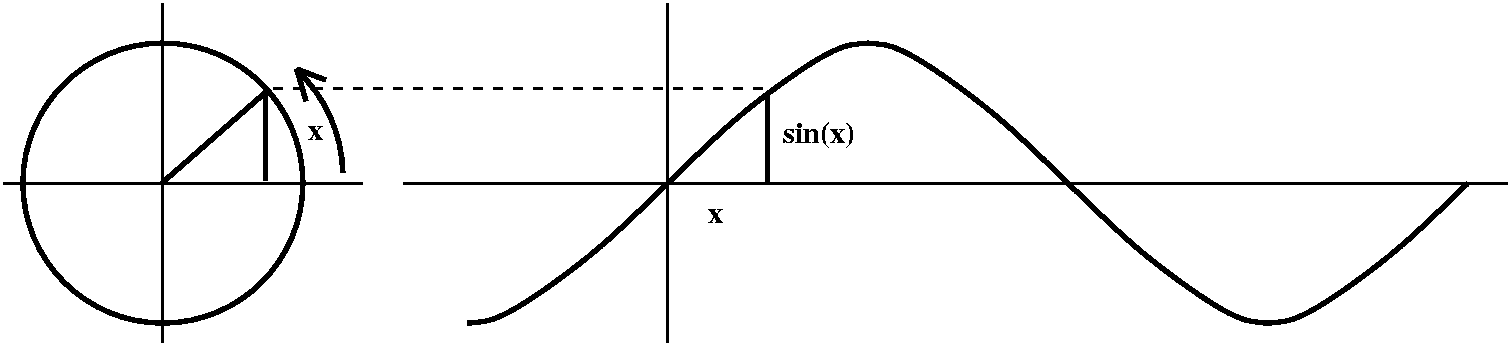
\includegraphics[width=\textwidth]{goniometriccircle_sine}
Breng ook eens een bezoekje aan \verb#http://www.geogebratube.org/student/m8028#, en wijzig daar $\theta$.

\begin{oefening}
Is ook de cosinusfunctie periodiek? Zo ja, bepaal dan de periode:
\arules{3}
\end{oefening}

\paragraph{Definitie}
\begin{mdframed}
Elke reële functie $f$ waarvoor geldt dat er een strikt positief getal $p$ bestaat waarvoor
$$\forall x+k\cdot p \in \mbox{dom} f: f(x)=f(x+k\cdot p)\qquad k\in\mathbb{Z}$$
noemen {\bf periodiek}. De kleinste positieve $p\in\mathbb{R}_0$ noemen we de {\bf periode} van de functie.
\end{mdframed}

\subsection{Amplitude van sinus- en cosinusfunctie}
Bij de sinus- en cosinusfunctie kunnen we de $x$-as als evenwichtsstand nemen. We merken dan op dat de functie steeds uitwijkt van de evenwichtsstand. We zullen de maximale uitwijking vanuit de evenwichtsstand de {\bf amplitude} A noemen.

\begin{oefening}
Bepaal de amplitude
\begin{enumerate}[(a)]
  \item van de sinusfunctie: \arulefill
  \item van de cosinusfunctie: \arulefill
\end{enumerate}
\end{oefening}

De amplitude kan van elke periodieke functie genomen worden die steeds uitwijkt ten opzichte van een evenwichtsstand.

\begin{oefening}
Bepaal voor volgende functie
\begin{center}
\definecolor{cqcqcq}{rgb}{0.7529411764705882,0.7529411764705882,0.7529411764705882}
\begin{tikzpicture}[scale=0.8,line cap=round,line join=round,>=triangle 45,x=1.0cm,y=1.0cm]
\draw [color=cqcqcq,, xstep=1.0cm,ystep=1.0cm] (-5.7606187437084495,-1.794685586926735) grid (5.594801414325579,3.4769983316916453);
\draw[->,color=black] (-5.7606187437084495,0.) -- (5.594801414325579,0.);
\foreach \x in {-5.,-4.,-3.,-2.,-1.,1.,2.,3.,4.,5.}
\draw[shift={(\x,0)},color=black] (0pt,2pt) -- (0pt,-2pt) node[below] {\footnotesize $\x$};
\draw[->,color=black] (0.,-1.794685586926735) -- (0.,3.4769983316916453);
\foreach \y in {-1.,1.,2.,3.}
\draw[shift={(0,\y)},color=black] (2pt,0pt) -- (-2pt,0pt) node[left] {\footnotesize $\y$};
\draw[color=black] (0pt,-10pt) node[right] {\footnotesize $0$};
\clip(-5.7606187437084495,-1.794685586926735) rectangle (5.594801414325579,3.4769983316916453);
\draw [line width=1.6pt] (-6.,3.)-- (-4.,3.);
\draw [line width=1.6pt] (-4.,-1.)-- (-2.,-1.);
\draw [line width=1.6pt] (-2.,3.)-- (0.,3.);
\draw [line width=1.6pt] (0.,-1.)-- (2.,-1.);
\draw [line width=1.6pt] (2.,3.)-- (4.,3.);
\draw [line width=1.6pt] (4.,-1.)-- (6.,-1.);
\end{tikzpicture}
\end{center}
\begin{enumerate}[(a)]
  \itemsep1em
  \item periode $P=\arule{3cm}$
  \item evenwichtsstand $\arule{5cm}$
  \item amplitude $A=\arule{3cm}$
\end{enumerate}
\end{oefening}

\begin{oefening}
Bepaal voor volgende functie
\begin{center}
\definecolor{cqcqcq}{rgb}{0.75,0.75,0.75}
\begin{tikzpicture}[scale=0.8,line cap=round,line join=round,>=triangle 45,x=1.0cm,y=1.0cm]
\draw [color=cqcqcq,dash pattern=on 1pt off 1pt, xstep=1.0cm,ystep=1.0cm] (-3.65,-2.55) grid (6.38,2.25);
\draw[->,color=black] (-3.65,0) -- (6.38,0);
\foreach \x in {-3,-2,-1,1,2,3,4,5,6}
\draw[shift={(\x,0)},color=black] (0pt,2pt) -- (0pt,-2pt) node[below] {\footnotesize $\x$};
\draw[->,color=black] (0,-2.55) -- (0,2.25);
\foreach \y in {-2,-1,1,2}
\draw[shift={(0,\y)},color=black] (2pt,0pt) -- (-2pt,0pt) node[left] {\footnotesize $\y$};
\draw[color=black] (0pt,-10pt) node[right] {\footnotesize $0$};
\clip(-3.65,-2.55) rectangle (6.38,2.25);
\draw[line width=2pt, smooth,samples=100,domain=-3.6545454545454543:6.381818181818182] plot(\x,{1.5*sin((3.1415926535*(\x))*180/pi)});
\end{tikzpicture}
\end{center}
\begin{enumerate}[(a)]
  \itemsep1em
  \item periode $P=\arule{3cm}$
  \item evenwichtsstand $\arule{5cm}$
  \item amplitude $A=\arule{3cm}$
\end{enumerate}
\end{oefening}

\begin{oefening}
Bepaal voor volgende functie
\begin{center}
\definecolor{cqcqcq}{rgb}{0.75,0.75,0.75}
\begin{tikzpicture}[line cap=round,line join=round,>=triangle 45,x=1.0cm,y=1.0cm]
\draw [color=cqcqcq,dash pattern=on 1pt off 1pt, xstep=1.0cm,ystep=1.0cm] (-2.42,-3.36) grid (12.26,2.26);
\draw[->,color=black] (-2.42,0) -- (12.26,0);
\foreach \x in {-2,-1,1,2,3,4,5,6,7,8,9,10,11,12}
\draw[shift={(\x,0)},color=black] (0pt,2pt) -- (0pt,-2pt) node[below] {\footnotesize $\x$};
\draw[->,color=black] (0,-3.36) -- (0,2.26);
\foreach \y in {-3,-2,-1,1,2}
\draw[shift={(0,\y)},color=black] (2pt,0pt) -- (-2pt,0pt) node[left] {\footnotesize $\y$};
\draw[color=black] (0pt,-10pt) node[right] {\footnotesize $0$};
\clip(-2.42,-3.36) rectangle (12.26,2.26);
\draw[line width=1.6pt, smooth,samples=100,domain=-2.4205950413223127:12.259404958677681] plot(\x,{2*sin((3.1415926535*(\x))*180/pi)+sin((2*3.1415926535*(\x)+1)*180/pi)});
\end{tikzpicture}
\end{center}
\begin{enumerate}[(a)]
  \itemsep1em
  \item periode $P=\arule{3cm}$
  \item evenwichtsstand $\arule{5cm}$
  \item amplitude $A=\arule{3cm}$
\end{enumerate}
\end{oefening}

\begin{oefening}
Bepaal voor volgende functie
\begin{center}
\definecolor{cqcqcq}{rgb}{0.75,0.75,0.75}
\begin{tikzpicture}[line cap=round,line join=round,>=triangle 45,x=1.0cm,y=1.0cm]
\draw [color=cqcqcq,dash pattern=on 1pt off 1pt, xstep=1.0cm,ystep=1.0cm] (-5.71,-1.49) grid (8.57,3.21);
\draw[->,color=black] (-5.71,0) -- (8.57,0);
\foreach \x in {-5,-4,-3,-2,-1,1,2,3,4,5,6,7,8}
\draw[shift={(\x,0)},color=black] (0pt,2pt) -- (0pt,-2pt) node[below] {\footnotesize $\x$};
\draw[->,color=black] (0,-1.49) -- (0,3.21);
\foreach \y in {-1,1,2,3}
\draw[shift={(0,\y)},color=black] (2pt,0pt) -- (-2pt,0pt) node[left] {\footnotesize $\y$};
\draw[color=black] (0pt,-10pt) node[right] {\footnotesize $0$};
\clip(-5.71,-1.49) rectangle (8.57,3.21);
\draw[line width=1.6pt, smooth,samples=100,domain=-5.705720690038618:8.570469617334128] plot(\x,{sin((1/2*3.1415926535*(\x))*180/pi)+cos((2*3.1415926535*(\x))*180/pi)+0.85});
\draw (-2.6,1.61) node[anchor=north west] {f};
\end{tikzpicture}
\end{center}
\begin{enumerate}[(a)]
  \itemsep1em
  \item periode $P=\arule{3cm}$
  \item evenwichtsstand $\arule{5cm}$
  \item amplitude $A=\arule{3cm}$
\end{enumerate}
\end{oefening}

\pagebreak
\subsection{De tangensfunctie}
\subsubsection{Tabel}
Vul onderstaande tabel aan. De hoek $x$ is uitgedrukt in radialen. Rond af op 2 decimalen.

\begin{adjustwidth}{-2.5cm}{-2.5cm}
\begin{center}
  \begin{tabular}{c|c|c|c|c|c|c|c|c|c|c}
    x & $\frac{-\pi}{2}$ &-1 & 0 & 1 &  $\frac{\pi}{2}$ & 2 & 3 & $\pi$ & 4 & $\frac{3\pi}{2}$ 
    \\
    \hline
   $\tan x$ &\hspace*{0.5cm}&\hspace*{0.5cm}&\hspace*{0.5cm}&\hspace*{0.5cm}&\hspace*{0.5cm}&\hspace*{0.5cm}&\hspace*{1cm}&\hspace*{0.5cm}&\hspace*{0.5cm}&\hspace*{0.5cm}
  \end{tabular}
\end{center}
\end{adjustwidth}


\subsubsection{Grafiek} 

\begin{center}
\definecolor{uququq}{rgb}{0.25,0.25,0.25}
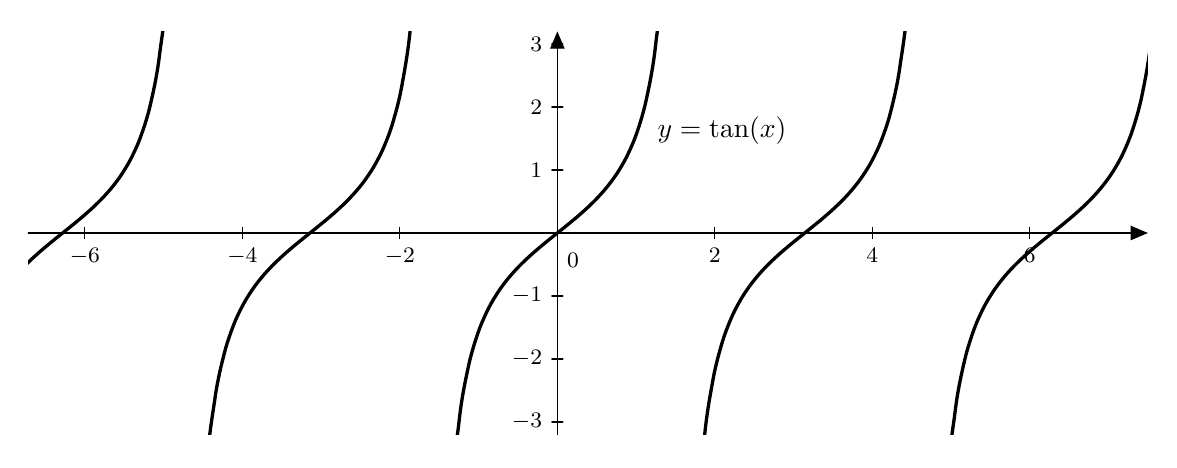
\begin{tikzpicture}[line cap=round,line join=round,>=triangle 45,x=1.0cm,y=.8cm]
\draw[->,color=black] (-6.72,0) -- (7.5,0);
\foreach \x in {-6,-4,-2,2,4,6}
\draw[shift={(\x,0)},color=black] (0pt,2pt) -- (0pt,-2pt) node[below] {\footnotesize $\x$};
\draw[->,color=black] (0,-3.2) -- (0,3.2);
\foreach \y in {-3,-2,-1,1,2,3}
\draw[shift={(0,\y)},color=black] (2pt,0pt) -- (-2pt,0pt) node[left] {\footnotesize $\y$};
\draw[color=black] (0pt,-10pt) node[right] {\footnotesize $0$};
\clip(-6.72,-3.2) rectangle (7.5,3.2);
\draw[line width=1.2pt, smooth, domain=-7.8:-4.8] plot (\x,{tan(\x*180/pi)});
\draw[line width=1.2pt, smooth, domain=-4.6:-1.6] plot (\x,{tan(\x*180/pi)});
\draw[line width=1.2pt, smooth, domain=-1.5:1.5] plot (\x,{tan(\x*180/pi)});
\draw[line width=1.2pt, smooth, domain=1.6:4.6] plot (\x,{tan(\x*180/pi)});
\draw[line width=1.2pt, smooth, domain=4.8:7.8] plot (\x,{tan(\x*180/pi)});
\draw[line width=1.2pt, smooth, domain=7.9:9] plot (\x,{tan(\x*180/pi)});
\draw (1.15,2) node[anchor=north west] {$y=\tan(x)$};
\end{tikzpicture}
\end{center}

\subsubsection{Kenmerken van de tangensfunctie}
\begin{oefening}
Vul de kenmerken aan van de cosinusfunctie.
\begin{enumerate}[(a)]
  \item $\dom \tan=\arule{3cm}$ en $\ber \tan=\arule{3cm}$
  \item Nulwaarden:
  \arules{3}
  \item Tekenverloop: 
  \begin{center}
    \visgraad{10cm}
  \end{center}
  \item Stijgen\&dalen en extreme waarden:
  \begin{center}
    \visgraad{10cm}
  \end{center}
  \item Periode: $p=\arule{3cm}$
\end{enumerate}
\end{oefening}

\newpage
\section{De algemene sinusfunctie}

\subsection{$\boldsymbol{f(x)=a\cdot\sin x}$ met $\boldsymbol{a\in \mathbb{R}^+_{0}}$}

\subsubsection{Voorbeeld: $\boldsymbol{y=3\cdot\sin x}$}


\begin{adjustwidth}{-2.5cm}{-2.5cm}
\begin{center}
\scriptsize
  \begin{tabular}{c|c|c|c|c|c|c|c|c|c|c|c|c}
    $x$ & -1 & 0 & 1 &  $\frac{\pi}{2}$ & 2 & 3 & $\pi$ & 4 & $\frac{3\pi}{2}$ & 5 & 6 & $2\pi$\\
    \hline
   $\sin x$ &-0.84&0&0.84&1&0.91&0.14&0&-0.76&-1&-0.96&-0.28 &0\\
    \hline
   $3\cdot\sin x$ &-2.52&0&2.52&3&2.73&0.42&0&-2.27&-3&-2.88&-0.84 &0
  \end{tabular}
\end{center}
\end{adjustwidth}

\begin{center}
\definecolor{cqcqcq}{rgb}{0.85,0.85,0.85}
\begin{tikzpicture}[line cap=round,line join=round,>=triangle 45,x=1.0cm,y=1.0cm]
\draw [color=cqcqcq,dash pattern=on 2pt off 2pt, xstep=1.0cm,ystep=1.0cm] (-2.9,-3.4) grid (9.4,3.4);
\draw[->,color=black] (-2.9,0) -- (9.4,0);
\foreach \x in {-2,-1,1,2,3,4,5,6,7,8,9}
\draw[shift={(\x,0)},color=black] (0pt,2pt) -- (0pt,-2pt) node[below] {\footnotesize $\x$};
\draw[->,color=black] (0,-3.4) -- (0,3.4);
\foreach \y in {-3,-2,-1,1,2,3}
\draw[shift={(0,\y)},color=black] (2pt,0pt) -- (-2pt,0pt) node[left] {\footnotesize $\y$};
\draw[color=black] (0pt,-10pt) node[right] {\footnotesize $0$};
\clip(-2.9,-3.4) rectangle (9.4,3.4);
\draw[color=gray, line width=1.2pt, smooth,samples=100,domain=-2.9:9.4] plot(\x,{sin(((\x))*180/pi)});
\draw[line width=1.2pt, smooth,samples=100,domain=-2.9:9.4] plot(\x,{3*sin(((\x))*180/pi)});
\begin{scriptsize}
\draw [color=gray] (1.58,1.46) node[anchor=north west] {$\sin(x)$};
\draw (2.4,2.53) node[anchor=north west] {$3\cdot \sin(x)$};
\end{scriptsize}
\end{tikzpicture}
\end{center}

\subsubsection{Verband tussen $\boldsymbol{y=\sin x}$ en $\boldsymbol{y=3\cdot\sin x}$}
De grafiek van $y=3\cdot\sin x$ bekom je door deze van $y=\sin x$ met een factor 3 verticaal uit te rekken. We spreken van een verschaling evenwijdig met de $y$-as met factor 3.\\
Hierdoor wordt de amplitude A met 3 vermenigvuldigd, terwijl de periode P gelijk blijft:
\begin{center}
  amplitude = A = 3\\
  periode = P = $2\pi$
\end{center}
\subsubsection{Algemeen}
{\bfseries
Voor $\boldsymbol{y=a\cdot\sin x}$ geldt:
  \begin{center}
    Grafiek van $\boldsymbol{y=\sin x}$ verschalen evenwijdig met de $y$-as met factor a:\\
    $\boldsymbol{a>1 \Rightarrow}$ uitrekking\\
    $\boldsymbol{a<1 \Rightarrow}$ inkrimping\\
    Amplitude $\boldsymbol{A = a}$\\
    Periode $\boldsymbol{P = 2\pi}$
  \end{center}
  }

\begin{oefening}
Geef telkens amplitude en periode van volgende functies.
\begin{center}
  \begin{tabular}{c|c|c|c|c}
     & $\sin x$ & $2\cdot\sin x$ &$\frac{1}{2}\cdot\sin x$ & $5\cdot\sin x$\\
    \hline
   Periode P &\arule{2cm} &\arule{2cm}&\arule{2cm}&\arule{2cm}
    \\
    \hline
   Amplitude A &\arule{2cm}&\arule{2cm}&\arule{2cm}&\arule{2cm}
  \end{tabular}
\end{center}
\end{oefening}

\subsection{$\boldsymbol{f(x)=\sin (b\cdot x)}$ met $\boldsymbol{b\in \mathbb{R}^+_{0}}$}
\subsubsection{Voorbeeld: $\boldsymbol{y=\sin (2x)}$}

\begin{adjustwidth}{-2.5cm}{-2.5cm}
\begin{center}
\scriptsize
  \begin{tabular}{c|c|c|c|c|c|c|c|c|c|c|c|c}
    x & -1 & 0 & 1 &  $\frac{\pi}{2}$ & 2 & 3 & $\pi$ & 4 & $\frac{3\pi}{2}$ & 5 & 6 & $2\pi$
    \\
    \hline
   $\sin x$ &-0.84&0&0.84&1&0.91&0.14&0&-0.76&-1&-0.96&-0.28 &0
    \\
    \hline
   $\sin (2x)$ &-0.91 &0 &0.91 &0 &-0.76 &-0.28 &0 &0.99 &0 &-0.54 &-0.54 &0
  \end{tabular}
\end{center}
\end{adjustwidth}

\begin{center}
\definecolor{cqcqcq}{rgb}{0.85,0.85,0.85}
\begin{tikzpicture}[line cap=round,line join=round,>=triangle 45,x=1.0cm,y=1.0cm]
\draw [color=cqcqcq,dash pattern=on 2pt off 2pt, xstep=1.0cm,ystep=1.0cm] (-2.9,-1.9) grid (9.4,1.9);
\draw[->,color=black] (-2.9,0) -- (9.4,0);
\foreach \x in {-2,-1,1,2,3,4,5,6,7,8,9}
\draw[shift={(\x,0)},color=black] (0pt,2pt) -- (0pt,-2pt) node[below] {\footnotesize $\x$};
\draw[->,color=black] (0,-1.9) -- (0,1.9);
\foreach \y in {-1,1}
\draw[shift={(0,\y)},color=black] (2pt,0pt) -- (-2pt,0pt) node[left] {\footnotesize $\y$};
\draw[color=black] (0pt,-10pt) node[right] {\footnotesize $0$};
\clip(-2.9,-1.9) rectangle (9.4,1.9);
\draw[color=gray, line width=1.2pt, smooth,samples=100,domain=-2.9:9.4] plot(\x,{sin(((\x))*180/pi)});
\draw[line width=1.2pt, smooth,samples=100,domain=-2.9:9.4] plot(\x,{sin((2*(\x))*180/pi)});
\begin{scriptsize}
\draw [color=gray] (1.0,1.46) node[anchor=north west] {$\sin(x)$};
\draw (2.80,1.46) node[anchor=north west] {$\sin(2x)$};
\end{scriptsize}
\end{tikzpicture}
\end{center}

\subsubsection{Verband tussen $\boldsymbol{y=\sin x}$ en $\boldsymbol{y=\sin (2x)}$}
De grafiek van $y=\sin (2x)$ bekom je door deze van $y=\sin x$ horizontaal samen te duwen. We spreken van een verschaling  evenwijdig met de $x$-as met factor $\frac{1}{2}$.\\
Hierdoor wordt de periode $P$ door $2$ gedeeld, terwijl de amplitude $A$ gelijk blijft:  
\begin{eqnarray*}
  \mbox{amplitude} &=& A = 1\\
  \mbox{periode} &=& P = \pi
\end{eqnarray*}

\subsubsection{Algemeen}
{\bfseries
Voor $\boldsymbol{y=\sin (bx)}$ geldt:
  \begin{center}
    Grafiek van $\boldsymbol{y=\sin x}$ verschalen evenwijdig met de $x$-as met factor $\boldsymbol{\frac{1}{b}}$:\\
    $\boldsymbol{b>1 \Rightarrow}$ inkrimping\\
    $\boldsymbol{0<b<1 \Rightarrow}$ uitrekking \\
    Amplitude $\boldsymbol{A = 1}$\\
    Periode $\boldsymbol{P = \frac{2\pi}{b}}$
  \end{center}
  }

\begin{oefening}
Geef telkens amplitude en periode van volgende functies.
\begin{center}
  \begin{tabular}{c|c|c|c|c}
     & $\sin x$ & $\sin (3x)$ &$\sin (\frac{1}{2}x)$ & $\sin (5x)$\\
    \hline
    Amplitude A &\hspace*{2cm} &\hspace*{2cm}&\hspace*{2cm}&\hspace*{2cm}
    \\
    \hline
    Periode P &\hspace*{2cm}&\hspace*{2cm}&\hspace*{2cm}&\hspace*{2cm}
  \end{tabular}
\end{center}
\end{oefening}

\subsection{$\boldsymbol{f(x)=\sin (x+c)}$ met $\boldsymbol{c\in \mathbb{R}}$}
\subsubsection{Voorbeeld: $\boldsymbol{y=\sin (x-1)}$}

\begin{adjustwidth}{-2.5cm}{-2.5cm}
\begin{center}
\scriptsize
  \begin{tabular}{c|c|c|c|c|c|c|c|c|c|c|c|c}
    x & -1 & 0 & 1 &  $\frac{\pi}{2}$ & 2 & 3 & $\pi$ & 4 & $\frac{3\pi}{2}$ & 5 & 6 & $2\pi$
    \\
    \hline
   $\sin x$ &-0.84&0&0.84&1&0.91&0.14&0&-0.76&-1&-0.96&-0.28 &0
    \\
    \hline
   $\sin (x-1)$ &-0.91 &-0.84 &0 &0.54 &0.84 &0.91 &0.84 &0.14 &-0.54 &-0.76 &-0.96 &-0.84
  \end{tabular}
\end{center}
\end{adjustwidth}

\begin{center}
\definecolor{cqcqcq}{rgb}{0.85,0.85,0.85}
\begin{tikzpicture}[line cap=round,line join=round,>=triangle 45,x=1.0cm,y=1.0cm]
\draw [color=cqcqcq,dash pattern=on 2pt off 2pt, xstep=1.0cm,ystep=1.0cm] (-2.9,-1.9) grid (9.4,1.9);
\draw[->,color=black] (-2.9,0) -- (9.4,0);
\foreach \x in {-2,-1,1,2,3,4,5,6,7,8,9}
\draw[shift={(\x,0)},color=black] (0pt,2pt) -- (0pt,-2pt) node[below] {\footnotesize $\x$};
\draw[->,color=black] (0,-1.9) -- (0,1.9);
\foreach \y in {-1,1}
\draw[shift={(0,\y)},color=black] (2pt,0pt) -- (-2pt,0pt) node[left] {\footnotesize $\y$};
\draw[color=black] (0pt,-10pt) node[right] {\footnotesize $0$};
\clip(-2.9,-1.9) rectangle (9.4,1.9);
\draw[color=gray, line width=1.2pt, smooth,samples=100,domain=-2.9:9.4] plot(\x,{sin(((\x))*180/pi)});
\draw[line width=1.2pt, smooth,samples=100,domain=-2.9:9.4] plot(\x,{sin(((\x -1))*180/pi)});
\begin{scriptsize}
\draw [color=gray] (1.0,1.46) node[anchor=north west] {$\sin(x)$};
\draw (2.80,1.46) node[anchor=north west] {$\sin(x-1)$};
\end{scriptsize}
\end{tikzpicture}
\end{center}

\subsubsection{Verband tussen $\boldsymbol{y=\sin x}$ en $\boldsymbol{y=\sin (x-1)}$}
De grafiek van $y=\sin (x-1)$ bekom je door deze van $y=\sin x$ horizontaal naar rechts te verschuiven met $1$ eenheid. We spreken van een verschuiving evenwijdig met de $x$-as, bepaald door het koppel $(1, 0)$.\\
Hierdoor blijven de periode $P$ en de amplitude $A$ gelijk.  
\begin{eqnarray*}
  \mbox{amplitude} &=& A = 1\\
  \mbox{periode} &=& P = 2\pi
\end{eqnarray*}

\subsubsection{Algemeen}
{\bfseries
Voor $\boldsymbol{y=\sin (x+c)}$ geldt:
  \begin{center}
    Grafiek van $\boldsymbol{y=\sin x}$ verschuiven evenwijdig met de $x$-as volgens het koppel $\boldsymbol{(-c, 0)}$:\\
    $\boldsymbol{c>0 \Rightarrow}$ c eenheden naar links\\
    $\boldsymbol{c<0 \Rightarrow}$ c eenheden naar rechts \\
    Amplitude $\boldsymbol{A = 1}$\\
    Periode $\boldsymbol{P = 2\pi}$
  \end{center}
  }

\begin{oefening}
Zeg telkens hoe je de grafiek van volgende functies kan bekomen uit deze van $y=\sin x$.
\begin{center}
  \begin{tabular}{c|c|c|c}
    $\sin (x-2)$ & $\sin (x-3)$ & $\sin (x+1)$ & $\sin (x+5)$\\
    \hline
    \hspace*{3cm} &\hspace*{3cm}&\hspace*{3cm}&\hspace*{3cm}
    \\
    &&&
    \\
    &&&
  \end{tabular}
\end{center}
\end{oefening}

\begin{oefening}
Hoe kan je de grafiek van volgende functies bekomen uit deze van de sinusfunctie?
\begin{enumerate}[(a)]
  \item $f(x)=\sin(x-2\pi)$
  \item $f(x)=\sin(x+2\pi)$
  \item $f(x)=\sin(x+4\pi)$
  \item $f(x)=\sin(x+2k\pi)$ met $k\in\mathbb{Z}$
\end{enumerate}
\end{oefening}

\subsection{$\boldsymbol{f(x)=\sin x + d}$ met $\boldsymbol{d\in \mathbb{R}}$} 
\subsubsection{Voorbeeld: $\boldsymbol{y=\sin x-1}$}
\begin{adjustwidth}{-2.5cm}{-2.5cm}
\begin{center}
\scriptsize
  \begin{tabular}{c|c|c|c|c|c|c|c|c|c|c|c|c}
    x & -1 & 0 & 1 &  $\frac{\pi}{2}$ & 2 & 3 & $\pi$ & 4 & $\frac{3\pi}{2}$ & 5 & 6 & $2\pi$
    \\
    \hline
   $\sin x$ &-0.84&0&0.84&1&0.91&0.14&0&-0.76&-1&-0.96&-0.28 &0
    \\
    \hline
   $\sin x-1$ &-1,84& -1& -0.16& 0& -0.09& -0.86& -1& -1,76& -2& -1,96& -1,28 &-1
  \end{tabular}
\end{center}
\end{adjustwidth}

\begin{center}
\definecolor{cqcqcq}{rgb}{0.85,0.85,0.85}
\begin{tikzpicture}[line cap=round,line join=round,>=triangle 45,x=1.0cm,y=1.0cm]
\draw [color=cqcqcq,dash pattern=on 2pt off 2pt, xstep=1.0cm,ystep=1.0cm] (-2.9,-2.9) grid (9.4,1.9);
\draw[->,color=black] (-2.9,0) -- (9.4,0);
\foreach \x in {-2,-1,1,2,3,4,5,6,7,8,9}
\draw[shift={(\x,0)},color=black] (0pt,2pt) -- (0pt,-2pt) node[below] {\footnotesize $\x$};
\draw[->,color=black] (0,-2.9) -- (0,1.9);
\foreach \y in {-1,1}
\draw[shift={(0,\y)},color=black] (2pt,0pt) -- (-2pt,0pt) node[left] {\footnotesize $\y$};
\draw[color=black] (0pt,-10pt) node[right] {\footnotesize $0$};
\clip(-2.9,-2.9) rectangle (9.4,1.9);
\draw[color=gray, line width=1.2pt, smooth,samples=100,domain=-2.9:9.4] plot(\x,{sin(((\x))*180/pi)});
\draw[line width=1.2pt, smooth,samples=100,domain=-2.9:9.4] plot(\x,{sin(((\x))*180/pi)-1});
\begin{scriptsize}
\draw [color=gray] (1.58,1.46) node[anchor=north west] {$\sin(x)$};
\draw (1.0,-0.46) node[anchor=north west] {$\sin(x)-1$};
\end{scriptsize}
\end{tikzpicture}
\end{center}

\subsubsection{Verband tussen $\boldsymbol{y=\sin x}$ en $\boldsymbol{y=\sin x-1}$}
De grafiek van $y=\sin x-1$ bekom je door deze van $y=\sin x$ verticaal naar beneden te verschuiven met 1 eenheid. We spreken van een verschuiving evenwijdig met de $y$-as, bepaald door het koppel $(0, -1)$.\\
Hierdoor blijven de periode $P$ en de amplitude $A$ gelijk.  
\begin{eqnarray*}
  \mbox{amplitude} &=& A = 1\\
  \mbox{periode} &=& P = 2\pi
\end{eqnarray*}

\subsubsection{Algemeen}
{\bfseries
Voor $\boldsymbol{y=\sin x+d}$ geldt:
  \begin{center}
    Grafiek van $\boldsymbol{y=\sin x}$ verschuiven evenwijdig met de $y$-as volgens het koppel $\boldsymbol{(0, d)}$:\\
    $\boldsymbol{d>0 \Rightarrow}$ d eenheden naar boven\\
    $\boldsymbol{d<0 \Rightarrow}$ d eenheden naar beneden \\
    Amplitude $\boldsymbol{A = 1}$\\
    Periode $\boldsymbol{P = 2\pi}$
  \end{center}
  }

\begin{oefening}
Zeg telkens hoe je de grafiek van volgende functies kan bekomen uit deze van $y=\sin x$.
\begin{center}
  \begin{tabular}{c|c|c|c}
    $\sin x-4$ & $\sin x-2$ & $\sin x+3$ & $\sin x+2$\\
    \hline
    \hspace*{3cm} &\hspace*{3cm}&\hspace*{3cm}&\hspace*{3cm}
    \\
    &&&
    \\
    &&&
  \end{tabular}
\end{center}
\end{oefening}

\subsection{De veralgemeende sinusfunctie $\boldsymbol{y=a\cdot \sin[b\cdot (x+c)]+d}$}

\begin{center}
  \fbox{\parbox{\linewidth}{
    {\bfseries
      De functie $\boldsymbol{y=a\cdot \sin[b\cdot (x+c)]+d}$ verloopt sinusoïdaal met\\
      \begin{itemize}
        \item Amplitude $\boldsymbol{A = a}$\\
        \item Periode $\boldsymbol{P=\dfrac{2\pi}{b}}$\\
      \end{itemize}  
      Je kan de grafiek ervan bekomen uit deze van $\boldsymbol{y=\sin x}$ door
      \begin{itemize}
        \item Een verschaling evenwijdig met de $y$-as met factor a\\
          $\boldsymbol{a>1 \Rightarrow}$ uitrekking\\
          $\boldsymbol{0<a<1 \Rightarrow}$ inkrimping\\
        \item Een verschaling evenwijdig met de $x$-as met factor $\boldsymbol{\dfrac{1}{b}}$\\
          $\boldsymbol{b>1 \Rightarrow}$ inkrimping\\
          $\boldsymbol{0<b<1 \Rightarrow}$ uitrekking \\
        \item Een verschuiving evenwijdig met de $x$-as bepaald door het koppel (-c, 0)\\
          $\boldsymbol{c>0 \Rightarrow}$ c eenheden naar links\\
          $\boldsymbol{c<0 \Rightarrow}$ c eenheden naar rechts \\
        \item Een verschuiving evenwijdig met de $y$-as bepaald door het koppel (0, d)\\
          $\boldsymbol{d>0 \Rightarrow}$ d eenheden naar boven\\
          $\boldsymbol{d<0 \Rightarrow}$ d eenheden naar beneden \\
      \end{itemize}}
    }}   
\end{center}
  
\begin{oefening}Bepaal amplitude A en periode P van volgende functies. Zeg telkens in woorden hoe je de grafiek kan bekomen uit deze van $y=\sin x$.\\
\begin{enumerate}[(a)]
  \item $y=\dfrac{1}{2}\cdot\sin [5\cdot(x+\dfrac{\pi}{8})]-3$
  \begin{itemize}
    \itemsep1em
    \item $a=\arule{2cm}\Rightarrow A=\arule{2cm}$
    \item $b=\arule{2cm}\Rightarrow P=\dfrac{2\pi}{b}=\arule{2cm}$
    \item $c=\arule{2cm}$
    \item $d=\arule{2cm}$
    \item Hoe bekom je de grafiek vanuit de sinusfunctie:
    \arules{3}
  \end{itemize}
  \item $\displaystyle y=3\cdot\sin\left(\dfrac{1}{2}x+\pi\right)-4$\\
  \begin{itemize}
    \itemsep1em
    \item $a=\arule{2cm}\Rightarrow A=\arule{2cm}$
    \item $b=\arule{2cm}\Rightarrow P=\dfrac{2\pi}{b}=\arule{2cm}$
    \item $c=\arule{2cm}$
    \item $d=\arule{2cm}$
    \item Hoe bekom je de grafiek vanuit de sinusfunctie:
    \arules{3}
  \end{itemize}
\end{enumerate}
\end{oefening}

\begin{oefening}Geef het voorschrift van de functie die men bekomt door de grafiek van $y=\sin x$
  \begin{enumerate}[(a)]
    \item
    \begin{enumerate}[$\rightarrow$]
      \itemsep0.8em
      \item te verschalen evenwijdig met de $y$-as met factor 2
      \item te verschalen evenwijdig met de $x$-as met factor 3
      \item te verschuiven evenwijdig met de $x$-as met 5 eenheden naar links
      \item te verschuiven evenwijdig met de $y$-as met 4 eenheden naar boven
    \end{enumerate}
    \arules{4}
    \item 
    \begin{enumerate}[$\rightarrow$]
      \itemsep0.8em
      \item te verschalen evenwijdig met de $y$-as met factor $\dfrac{1}{4}$
      \item te verschalen evenwijdig met de $x$-as met factor $\dfrac{1}{5}$
      \item te verschuiven evenwijdig met de $x$-as met 2 eenheden naar rechts
      \item te verschuiven evenwijdig met de $y$-as met 6 eenheden naar beneden
    \end{enumerate}
    \arules{4}
  \end{enumerate}
\end{oefening}

\pagebreak
\section{Goniometrische vergelijkingen}

\subsection{De goniometrische vergelijking $\sin x=r$}
Goniometrische vergelijkingen kunnen op twee manieren opgelost worden, aan de hand van de grafiek van de sinusfunctie of m.b.v. de rekenmachine. We illustreren beide manieren met een voorbeeld.

\subsubsection{Grafische oplossingsmethode}
\paragraph*{Voorbeeld:} $$\sin x = 0.5$$
Snijd je de grafiek van $y=\sin x$ met de rechte $y=0.5$, dan vind je oneindig veel snijpunten. De $x$-coördinaten van al deze snijpunten vormen de oplossingen van de vergelijking.\\

\begin{center}
\definecolor{uququq}{rgb}{0.25,0.25,0.25}
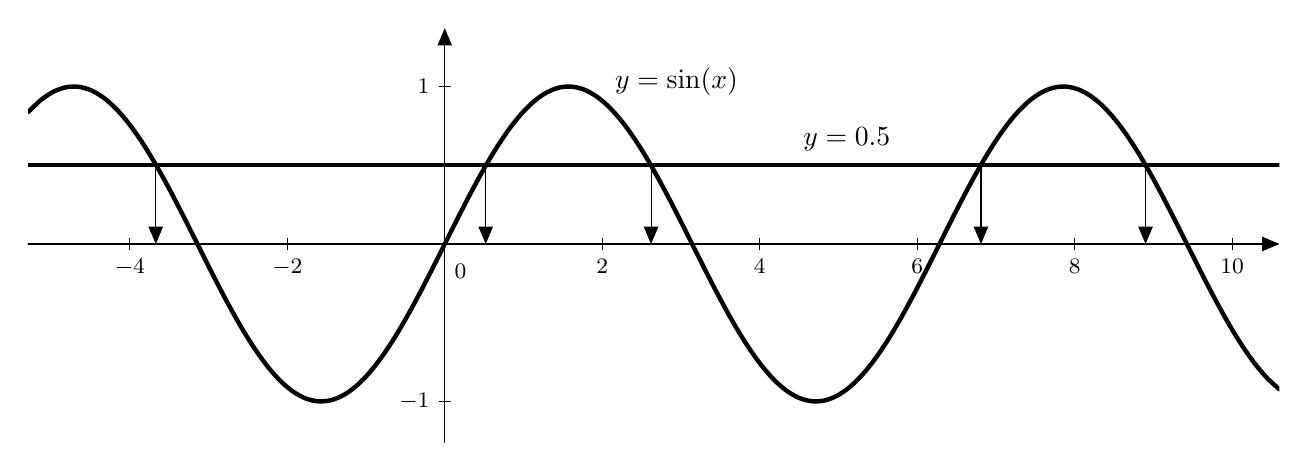
\begin{tikzpicture}[line cap=round,line join=round,>=triangle 45,x=1.0cm,y=2.0cm]
\draw[->,color=black] (-5.29,0) -- (10.6,0);
\foreach \x in {-4,-2,2,4,6,8,10}
\draw[shift={(\x,0)},color=black] (0pt,2pt) -- (0pt,-2pt) node[below] {\footnotesize $\x$};
\draw[->,color=black] (0,-1.26) -- (0,1.37);
\foreach \y in {-1,1}
\draw[shift={(0,\y)},color=black] (2pt,0pt) -- (-2pt,0pt) node[left] {\footnotesize $\y$};
\draw[color=black] (0pt,-10pt) node[right] {\footnotesize $0$};
\clip(-5.29,-1.26) rectangle (10.6,1.37);
\draw[line width=1.6pt, smooth,samples=100,domain=-5.2882192996279604:10.601096701140744] plot(\x,{sin(((\x))*180/pi)});
\draw (2.04,1.18) node[anchor=north west] {$y=\sin(x)$};
\draw[line width=1.6pt, smooth,samples=100,domain=-5.2882192996279604:10.601096701140744] plot(\x,{0.5});
\draw (4.43,0.8) node[anchor=north west] {$y=0.5$};
\draw [->] (-3.67,0.5)-- (-3.67,0);
\draw [->] (0.52,0.5)-- (0.52,0);
\draw [->] (2.62,0.5)-- (2.62,0);
\draw [->] (6.81,0.5)-- (6.81,0);
\draw [->] (8.9,0.5)-- (8.9,0);
\end{tikzpicture}
\end{center}
\arules{9}

\pagebreak
\subsubsection{Gebruik van de ZRM}
\paragraph*{Voorbeeld:}
$$\sin x = 0.85$$
Indien de $x$-waarde van de snijpunten niet makkelijk af te lezen valt op de grafiek, kunnen we beter gebruik maken van onze rekenmachine.
Hiertoe voer je volgende stappen uit.
\begin{itemize}
  \item Zet je ZRM in de radialen-modus.
  \item Typ $0.85$ en vervolgens \zrm{SHIFT} \zrm{$\sin^{-1}$}.\\
  Dit geeft ons als resultaat \arulefill
  De ZRM geeft dus één oplossing, nl. $x_{1}=1.016$. 
  \item De eerste reeks vind je met een analoge redenering als bij de grafische methode: telkens je een geheel veelvoud van $2\pi$ bij de gevonden $x$-waarde optelt, krijg je een nieuwe oplossing:
  $$x_{1,k}=1.016+k\cdot2\pi \mbox{ met } k \in \mathbb{Z}$$
  \item De tweede reeks oplossingen vind je door gebruik te maken van verwante hoeken.\\
  {\bf Supplementaire hoeken}, hoeken met som $\pi$, hebben namelijk gelijke sinussen.\\
  Als $x_{1}=1,016$ een oplossing is, dan is de supplementaire hoek 
  \begin{eqnarray*}
  x_2 &=& \pi -x_{1}\\
      &=& \pi - 1.016\\
      &=& 2.1256
  \end{eqnarray*}
  ook een oplossing. En wegens de periodiciteit van de sinusfunctie krijgen we ook hier een tweede reeks oplossingen:
  $$x_{2,k} = 2.1256+k\cdot2\pi \mbox{ met } k \in \mathbb{Z}$$
  \item De oplossingenverzameling $$V = \{\arule{10cm}\}$$
\end{itemize}


\begin{oefening}
Los op in $\mathbb{R}$ met een methode naar keuze.
\begin{enumerate}[(a)]
  \item $\sin x=1$
  \arules{6}
  \item $\sin x=\dfrac{-\sqrt{3}}{2}$
  \arules{6}
  \item $\sin x=-0.96$
  \arules{6}
  \item $\sin x=1.001$
  \arules{6}
\end{enumerate}
\end{oefening}

\pagebreak
\subsection{De goniometrische vergelijking $\cos x=r$}
We illustreren ook hier beide manieren met een voorbeeld.

\subsubsection{Grafische oplossingsmethode}

\paragraph*{Voorbeeld:}
$$\cos x = 0.5$$
Snijd je de grafiek van $y=\cos x$ met de rechte $y=0.5$, dan vind je oneindig veel snijpunten. De $x$-coördinaten van al deze snijpunten vormen de oplossingen van de vergelijking.\\
\begin{center}
\definecolor{uququq}{rgb}{0.25,0.25,0.25}
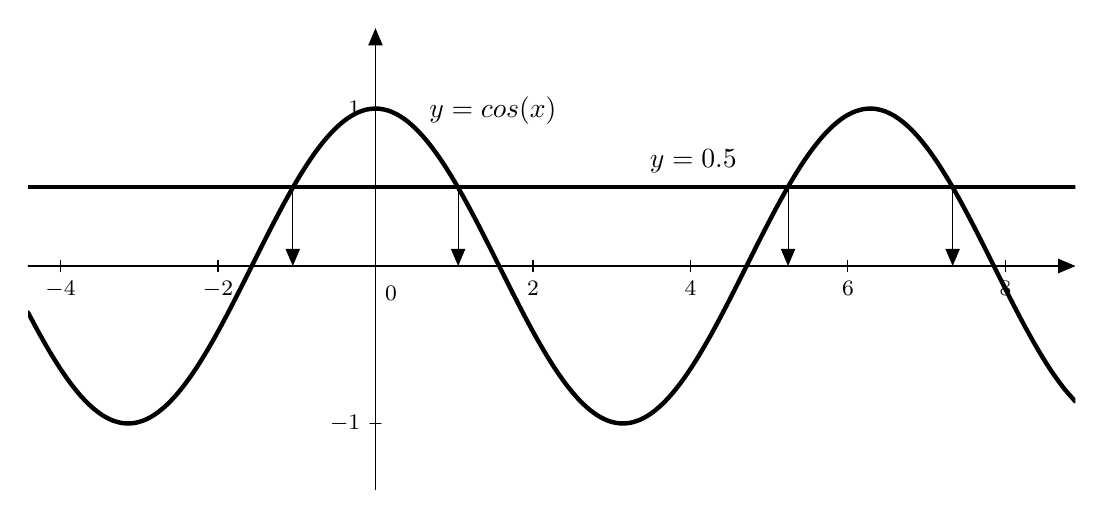
\begin{tikzpicture}[line cap=round,line join=round,>=triangle 45,x=1.0cm,y=2.0cm]
\draw[->,color=black] (-4.41,0) -- (8.89,0);
\foreach \x in {-4,-2,2,4,6,8}
\draw[shift={(\x,0)},color=black] (0pt,2pt) -- (0pt,-2pt) node[below] {\footnotesize $\x$};
\draw[->,color=black] (0,-1.42) -- (0,1.51);
\foreach \y in {-1,1}
\draw[shift={(0,\y)},color=black] (2pt,0pt) -- (-2pt,0pt) node[left] {\footnotesize $\y$};
\draw[color=black] (0pt,-10pt) node[right] {\footnotesize $0$};
\clip(-4.41,-1.42) rectangle (8.89,1.51);
\draw[line width=1.6pt, smooth,samples=100,domain=-4.412379644059984:8.885821483268002] plot(\x,{cos(((\x))*180/pi)});
\draw (0.56,1.14) node[anchor=north west] {$y=cos(x)$};
\draw[line width=1.6pt, smooth,samples=100,domain=-4.412379644059984:8.885821483268002] plot(\x,{0.5});
\draw (3.36,0.8) node[anchor=north west] {$y=0.5$};
\draw [->] (-5.24,0.5)-- (-5.24,0);
\draw [->] (-1.05,0.5)-- (-1.05,0);
\draw [->] (1.05,0.5)-- (1.05,0);
\draw [->] (5.24,0.5)-- (5.24,0);
\draw [->] (7.33,0.5)-- (7.33,0);
\end{tikzpicture}
\end{center}
\arules{8}

\pagebreak
\subsubsection{Gebruik van de ZRM}

\paragraph*{Voorbeeld:}
$$\cos x = 0.85$$
\begin{itemize}
  \item Zet je ZRM in de radialen-modus.
  \item Typ $0.85$ en vervolgens \zrm{SHIFT} \zrm{$\cos^{-1}$}.\\
  Dit geeft ons als resultaat \arulefill
  De ZRM geeft dus één oplossing, nl. $x_{1}=0.5548$. 
  \item De eerste reeks vind je met een analoge redenering als bij de grafische methode: telkens je een geheel veelvoud van $2\pi$ bij de gevonden $x$-waarde optelt, krijg je een nieuwe oplossing
  $$x_{1,k}=0.5548+k\cdot2\pi \mbox{ met } k \in \mathbb{Z}$$
  \item De tweede reeks oplossingen vind je door gebruik te maken van verwante hoeken.\\
  \textbf{Tegengestelde hoeken}, hoeken met een gelijke absolute waarde maar met een tegengesteld teken, hebben namelijk gelijke cosinussen.\\
  Als $x_{1}=0.5548$ een oplossing is, dan is de tegengestelde hoek $x_2=-x_1=-0.5548$ ook een oplossing. En wegens de peiodiciteit van de cosinusfunctie krijgen we ook hier een tweede reeks oplossingen:\\
  $$x_{2,k}=-0.5548+k\cdot 2\pi \mbox{ met } k \in \mathbb{Z}$$
  \item De oplossingenverzameling 
  $$V = \{\arule{10cm}\}$$
\end{itemize}

\begin{oefening}
Los op in $\mathbb{R}$ met een methode naar keuze.
\begin{enumerate}[(a)]
  \item $\cos x=\frac{1}{2}$
  \arules{6}
  \item $\cos x=\frac{\sqrt{3}}{2}$
  \arules{6}
  \item $\cos x=-0.29$
  \arules{6}
  \item $\cos x=-1.1$
  \arules{6}
\end{enumerate}
\end{oefening}

\subsection{De goniometrische vergelijking $\tan x=r$}

\subsubsection{Grafische oplossingsmethode}
\paragraph*{Voorbeeld:}
$$\tan x = 0.5$$
Snijd je de grafiek van $y=\tan x$ met de rechte $y=0.5$, dan vind je oneindig veel snijpunten. De $x$-coördinaten van al deze snijpunten vormen de oplossingen van de vergelijking.\\
\begin{center}
\definecolor{uququq}{rgb}{0.25,0.25,0.25}
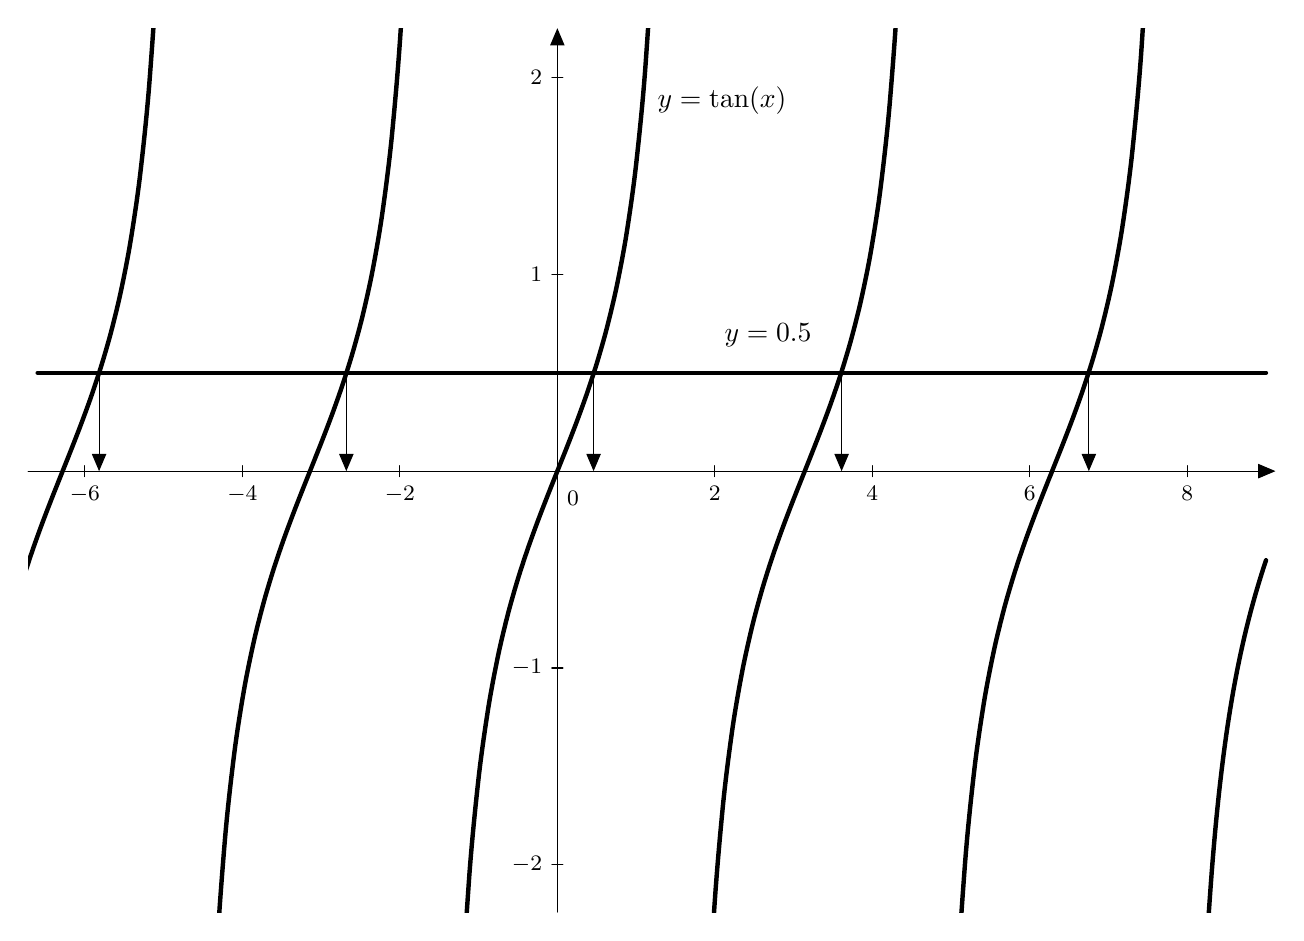
\begin{tikzpicture}[line cap=round,line join=round,>=triangle 45,x=1.0cm,y=2.5cm]
\draw[->,color=black] (-6.72,0) -- (9.12,0);
\foreach \x in {-6,-4,-2,2,4,6,8}
\draw[shift={(\x,0)},color=black] (0pt,2pt) -- (0pt,-2pt) node[below] {\footnotesize $\x$};
\draw[->,color=black] (0,-2.24) -- (0,2.25);
\foreach \y in {-2,-1,1,2}
\draw[shift={(0,\y)},color=black] (2pt,0pt) -- (-2pt,0pt) node[left] {\footnotesize $\y$};
\draw[color=black] (0pt,-10pt) node[right] {\footnotesize $0$};
\clip(-6.72,-2.24) rectangle (9.12,2.25);
\draw[line width=1.6pt, smooth, domain=-7.8:-4.8] plot (\x,{tan(\x*180/pi)});
\draw[line width=1.6pt, smooth, domain=-4.6:-1.6] plot (\x,{tan(\x*180/pi)});
\draw[line width=1.6pt, smooth, domain=-1.5:1.5] plot (\x,{tan(\x*180/pi)});
\draw[line width=1.6pt, smooth, domain=1.6:4.6] plot (\x,{tan(\x*180/pi)});
\draw[line width=1.6pt, smooth, domain=4.8:7.8] plot (\x,{tan(\x*180/pi)});
\draw[line width=1.6pt, smooth, domain=7.9:9] plot (\x,{tan(\x*180/pi)});
\draw (1.15,2) node[anchor=north west] {$y=\tan(x)$};
\draw[line width=1.6pt, smooth,samples=100,domain=-6.6:9.0] plot(\x,{0.5});
\draw (2.0,0.8) node[anchor=north west] {$y=0.5$};
\draw [->] (-5.82,0.5)-- (-5.82,0);
\draw [->] (0.46,0.5)-- (0.46,0);
\draw [->] (6.75,0.5)-- (6.75,0);
\draw [<-] (-2.68,0)-- (-2.68,0.5);
\draw [<-] (3.61,0)-- (3.61,0.5);
\end{tikzpicture}
\end{center}
\arules{6}

\pagebreak
\subsubsection{Gebruik van de ZRM}
\paragraph*{Voorbeeld:}
$$\tan x = -3$$
Indien de $x$-waarde van de snijpunten niet makkelijk af te lezen valt op de grafiek, kunnen we beter gebruik maken van onze rekenmachine.
Hiertoe voer je volgende stappen uit.
\begin{itemize}
  \item Zet je ZRM in de radialen-modus.
  \item Typ -3 en vervolgens \zrm{SHIFT} \zrm{$\tan ^{-1}$}.\\
  Dit geeft ons als resultaat \arulefill
  De ZRM geeft dus één oplossing, nl. $x_{0}=-1.25$. 
  \item Telkens je een geheel veelvoud van $\pi$ bij de gevonden $x$-waarde optelt, krijg je een nieuwe oplossing
  $$x_k=-1.25+k\cdot\pi \mbox{ met } k \in \mathbb{Z}$$
  \item De oplossingenverzameling
  $$V = \{\arule{8cm}\}$$
\end{itemize}

\begin{oefening}
Los op in $\mathbb{R}$ met een methode naar keuze.
\begin{enumerate}[(a)]
  \item $\tan x=0$
  \arules{2}
  \item $\tan x=\frac{1}{\sqrt{3}}$
  \arules{2}
  \item $\tan x=25$
  \arules{2}
  \item $\tan x=-0.25$
  \arules{2}
\end{enumerate}
\end{oefening}

\begin{oefening}
Bepaal \textbf{zonder} ZRM elke hoek $\alpha$ waarvoor geldt
\begin{enumerate}[(a)]
  \item $\sin\alpha=\frac{1}{2}$\arules{2}
  \item $\sin\alpha=-1$\arules{2}
  \item $\sin\alpha=0$\arules{2}
  \item $\cos\alpha=\frac{\sqrt{2}}{2}$\arules{2}
  \item $\cos\alpha=1$\arules{2}
  \item $\cos\alpha=0$\arules{2}
  \item $\tan\alpha=\sqrt{3}$\arules{2}
  \item $\tan\alpha=1$\arules{2}
  \item $\tan\alpha=-1$\arules{2}
\end{enumerate}
\end{oefening}

\begin{oefening}
Bepaal \textbf{met} ZRM elke hoek $\alpha$ waarvoor geldt
\begin{enumerate}[(a)]
  \item $\sin\alpha=0.4$\arules{2}
  \item $\sin\alpha=-0.72$\arules{2}
  \item $\sin\alpha=-2$\arules{2}
  \item $\cos\alpha=0.943$\arules{2}
  \item $\cos\alpha=0.666$\arules{2}
  \item $\tan\alpha=7$\arules{2}
  \item $\tan\alpha=5\pi$\arules{2}
  \item $\tan\alpha=-14$\arules{2}
\end{enumerate}
\end{oefening}

\pagebreak
\section{Toepassingen}

\begin{oefening}\\
De verkoop van badpakken is seizoensgebonden. Uit onderzoek weet een bedrijf dat in de $t$-de week van het jaar een winst $W$ in honderden euro's realiseert, gegeven door de formule
$$W=4-4\cos\left(\dfrac{\pi}{26}t\right) \mbox{ met } t\in \{1,2,3,\ldots,51,52\}$$
\begin{enumerate}[(a)]
  \item Bereken de winst $W$ voor $t=13$.
    \arules{2}
  \item Bereken de winst $W$ voor $t=26$.
    \arules{2}  
  \item Bereken de winst $W$ voor $t=50$.
    \arules{2}
\end{enumerate}
\end{oefening}

\begin{oefening}\\
De verkoop van frisdranken is eveneens seizoensgebonden. Een bedrijf gebruikt de volgende formule om de inkomsten $I$ (in miljoenen euro) te schatten in de t-de maand van het jaar:
$$I=5-4\cos\left(\dfrac{\pi}{6}t\right) \mbox{ met } t\in \{1,2,3,...,11,12\}$$
\begin{enumerate}[(a)]
  \item Bereken de inkomsten voor $t=2$.
    \arules{2}
  \item Bereken de inkomsten voor $t=3$.
    \arules{2}  
  \item Bereken de inkomsten voor $t=6$.
    \arules{2}
\end{enumerate}
\end{oefening}

\begin{oefening}\\
Sommige mensen geloven dat het leven van een mens verloopt in cycli van goede en slechte dagen. Ze onderscheiden drie cycli, bioritmen genoemd, die alle beginnen bij de geboorte.
\begin{itemize}
  \item fysiek bioritme (vitaliteit, sterkte, energie), voorgesteld door een sinusfunctie met een periode van 23 dagen:\\
    $y=\sin\left(\dfrac{2\pi}{23}t\right)$
   \item emotioneel bioritme (creativiteit, stemming, welbehagen), voorgesteld door een sinusfunctie met een periode van 28 dagen:\\
    $y=\sin\left(\dfrac{2\pi}{28}t\right)$ 
   \item intellectueel bioritme (hersenarbeid, inzicht, studiebereidheid, geheugen), voorgesteld door een sinusfunctie met een periode van 33 dagen:\\
    $y=\sin\left(\dfrac{2\pi}{33}t\right)$ 
\end{itemize}
Voor $y=1$ is het betreffende bioritme uiterst gunstig; voor $y=-1$ uiterst ongunstig.\\
\begin{enumerate}[(a)]
  \item Beschrijf de toestand 5537 dagen na de geboorte. Dat is afhankelijk van het aantal verlopen schrikkeljaren 15 jaar en 58 dagen of 15 jaar en 59 dagen.
    \arules{4}
  \item Bepaal je leeftijd in dagen en bereken de huidige toestand van je bioritmen.
    \arules{12}
\end{enumerate}
\end{oefening}



%Vanaf hier voor 5ELME en 5MT +2u

\section{Goniometrische getallen van enkele bijzondere hoeken}
\begin{center}
  \begin{tabular}{c|c|c|c|c|c|c|c|c|c}
    $x$ & $0$ & $\frac{\pi}{6}$ & $\frac{\pi}{4}$ &$\frac{\pi}{3}$ &$\frac{\pi}{2}$ &$\frac{2\pi}{3}$ &$\frac{3\pi}{4}$ &$\frac{5\pi}{6}$ & $\pi$ \\
    \hline
    $\sin x$&&&&&&&&&\\
    \hline
    $\cos x$&&&&&&&&&\\
    \hline
    $\tan x$&&&&&&&&&\\ 
  \end{tabular}
  \vfill
  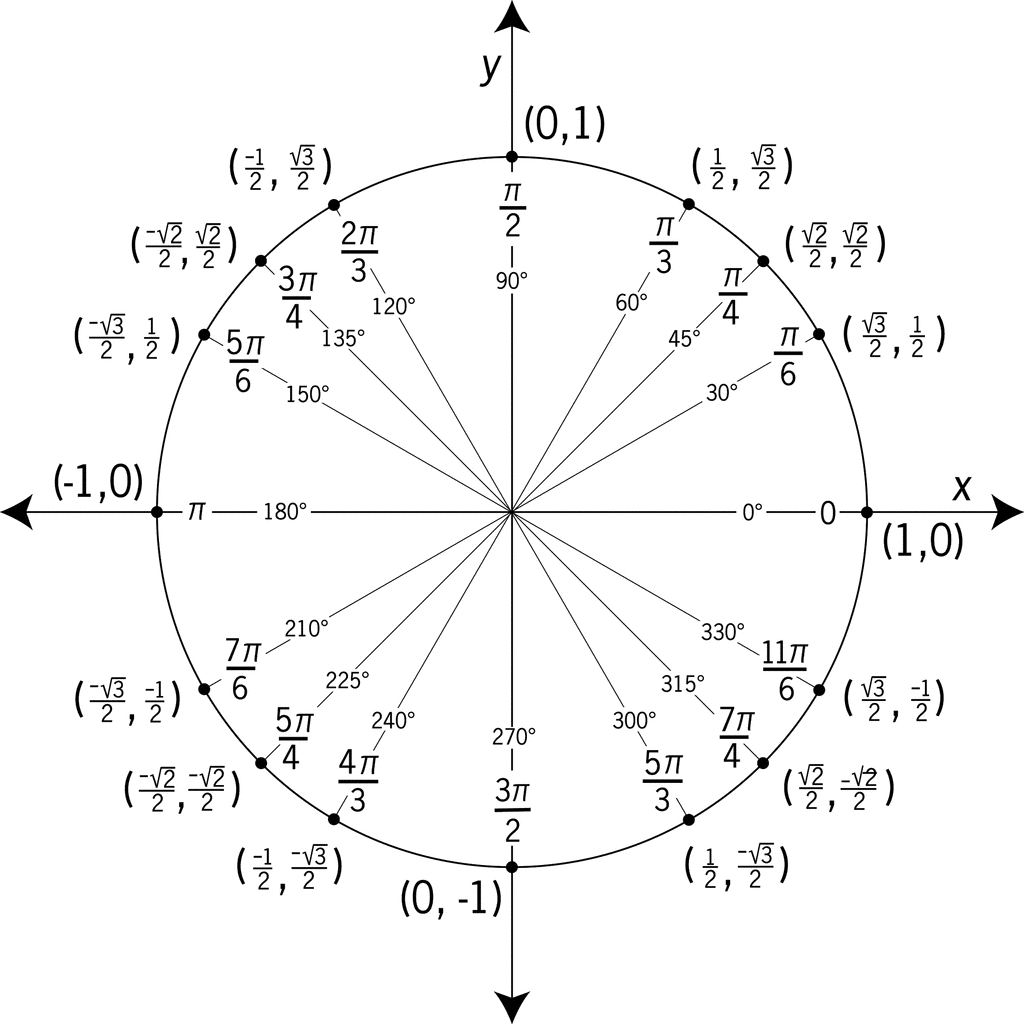
\includegraphics[width=0.8\textwidth]{unit-circle} %% SOURCE: http://etc.usf.edu
  \vfill
\end{center}


\pagebreak
\section{Goniometrische getallen van verwante hoeken}

\subsection{Gelijke hoeken}
We noemen twee hoeken $\alpha$ en $\beta$ \textbf{gelijk} als \arulefill
\paragraph{}
Aangezien $2\pi$ de periode is van de sinus- en cosinusfunctie, zullen gelijke hoeken dezelfde goniometrische getallen hebben.
\[\sin(\alpha+k.2\pi)=\sin(\alpha)
\]
\[\cos(\alpha +k.2\pi)=\cos(\alpha)
\]
\[\tan(\alpha+k.2\pi)=\tan(\alpha)
\]
\[\cot(\alpha +k.2\pi)=\cot(\alpha)
\]

\subsection{Tegengestelde hoeken}
\subsubsection{Definitie}
We noemen twee hoeken $\alpha$ en $\beta$ \textbf{tegengesteld} als \arulefill
\subsubsection{Goniometrische getallen van tegengestelde hoeken}
Teken hieronder een goniometrische cirkel en lees erop af wat het verband is tussen $\sin(\alpha)$ en $\sin(-\alpha)$. Doe hetzelfde voor cos, tan en cot.
\vspace*{3cm}
\subsubsection{Besluit}
\[\sin(-\alpha)=-\sin(\alpha)
\]
\[\cos(-\alpha)=\cos(\alpha)
\]
\[\tan(-\alpha)=-\tan(\alpha)
\]
\[\cot(-\alpha)=-\cot(\alpha)
\]

\subsection{Complementaire hoeken}
\subsubsection{Definitie}
We noemen twee hoeken $\alpha$ en $\beta$ \textbf{complementair} als \arulefill
\subsubsection{Goniometrische getallen van complementaire hoeken}
Teken hieronder een goniometrische cirkel en lees erop af wat het verband is tussen $\sin(\alpha)$ en $\sin(\frac{\pi}{2}-\alpha)$. Doe hetzelfde voor cos, tan en cot.
\vspace*{7cm}
\subsubsection{Besluit}
\[\sin(\frac{\pi}{2}-\alpha)=\cos(\alpha)
\]
\[\cos(\frac{\pi}{2}-\alpha)=\sin(\alpha)
\]
\[\tan(\frac{\pi}{2}-\alpha)=\cot(\alpha)
\]
\[\cot(\frac{\pi}{2}-\alpha)=\tan(\alpha)
\]

\subsection{Supplementaire hoeken}
\subsubsection{Definitie}
We noemen twee hoeken $\alpha$ en $\beta$ \textbf{supplementair} als \arulefill
\subsubsection{Goniometrische getallen van supplementaire hoeken}
Teken hieronder een goniometrische cirkel en lees erop af wat het verband is tussen $\sin(\alpha)$ en $\sin(\pi-\alpha)$. Doe hetzelfde voor cos, tan en cot.
\vspace*{7cm}
\subsubsection{Besluit}
\[\sin(\pi-\alpha)=\sin(\alpha)
\]
\[\cos(\pi-\alpha)=-\cos(\alpha)
\]
\[\tan(\pi-\alpha)=-\tan(\alpha)
\]
\[\cot(\pi-\alpha)=-\cot(\alpha)
\]

\subsection{Antisupplementaire hoeken}
\subsubsection{Definitie}
We noemen twee hoeken $\alpha$ en $\beta$ \textbf{antisupplementair} als \arulefill
\subsubsection{Goniometrische getallen van antisupplementaire hoeken}
Teken hieronder een goniometrische cirkel en lees erop af wat het verband is tussen $\sin(\alpha)$ en $\sin(\pi+\alpha)$. Doe hetzelfde voor cos, tan en cot.
\vspace*{6cm}
\subsubsection{Besluit}
\[\sin(\pi+\alpha)=-\sin(\alpha)
\]
\[\cos(\pi+\alpha)=-\cos(\alpha)
\]
\[\tan(\pi+\alpha)=\tan(\alpha)
\]
\[\cot(\pi+\alpha)=\cot(\alpha)
\]
\subsection{Herhaling formules uit de tweede graad}
\[\cos^{2}\alpha+\sin^{2}\alpha=1\]
\[\tan\alpha=\frac{\sin\alpha}{\cos\alpha}=\frac{1}{\cot\alpha}\]
\[\cot\alpha=\frac{\cos\alpha}{\sin\alpha}=\frac{1}{\tan\alpha}\]
\[1+\tan^{2}\alpha=\frac{1}{\cos^{2}\alpha}\]
\[1+\cot^{2}\alpha=\frac{1}{\sin^{2}\alpha}\]

\newpage
\subsection{Oefeningen}
\underline{Gegeven is dat de volgende vormen zinvol zijn. Schrijf ze zo eenvoudig mogelijk}

\begin{enumerate}[(a)]
  \item $\frac{\cos(\frac{\pi}{2}-\alpha)}{\tan(\pi+\alpha)}=$ \arules{2}
  \item $\frac{\sin(\frac{\pi}{2}-\alpha)}{\cot(\pi-\alpha)}=$ \arules{2}
  \item $\frac{sin(\pi+\alpha).\tan(\pi-\alpha)}{\tan(-\alpha)}=$ \arules{2}
  \item $(1-\cos(-\alpha)).(1+cos(\alpha))=$ \arules{2}
  \item $\frac{sin(\frac{\pi}{2}-\alpha).\cos(2\pi+\alpha).\cot(\frac{\pi}{2}-\alpha)}{\tan(\pi-\alpha).\cot(\alpha+\pi).\cos(-\alpha)}=$ \arules{2}
\end{enumerate}

\end{document}
\newpage
\section{Optellingsformules}

\subsection{Inleiding}
We willen een formule afleiden om de sinus, cosinus of tangens van een som van twee hoeken te berekenen: 
\[\sin(\alpha + \beta)
\]
\[\cos(\alpha + \beta)
\]
\[\tan(\alpha+\beta)
\]
Vul hiertoe de volgende uitdrukkingen aan en verbind wat aan elkaar gelijk is.
\[\sin(\frac{\pi}{6} + \frac{\pi}{3})=\sin(\frac{\pi}{2})=.........................
\]
\[\sin(\frac{\pi}{6}) + \sin(\frac{\pi}{3})=..............................
\]
\[\sin(\frac{\pi}{6}).\cos(\frac{\pi}{3})+\cos(\frac{\pi}{6}).\sin(\frac{\pi}{3})=..........................................
\]
\paragraph{}
\[\sin(\frac{\pi}{2} - \frac{\pi}{6})=\sin(\frac{\pi}{3})=.........................
\]
\[\sin(\frac{\pi}{2}) - \sin(\frac{\pi}{6})=..............................
\]
\[\sin(\frac{\pi}{2}).\cos(\frac{\pi}{6})-\cos(\frac{\pi}{2}).\sin(\frac{\pi}{6})=..........................................
\]
\paragraph{}
\[\cos(\frac{\pi}{6} + \frac{\pi}{3})=\cos(\frac{\pi}{2})=.........................
\]
\[\cos(\frac{\pi}{6}) + \cos(\frac{\pi}{3})=..............................
\]
\[\cos(\frac{\pi}{6}).\cos(\frac{\pi}{3}) - \sin(\frac{\pi}{6}).\sin(\frac{\pi}{3})=..........................................
\]
\paragraph{}
\[\cos(\frac{\pi}{2} - \frac{\pi}{6})=\cos(\frac{\pi}{3})=.........................
\]
\[\cos(\frac{\pi}{2}) - \cos(\frac{\pi}{6})=..............................
\]
\[\cos(\frac{\pi}{2}).\cos(\frac{\pi}{6}) + \sin(\frac{\pi}{2}).\sin(\frac{\pi}{6})=..........................................
\]



\subsection{Besluit: Optellingsformules voor sinus en cosinus}

\textbf{\[\sin(\alpha + \beta)=\sin(\alpha)\cdot \cos(\beta)+\cos(\alpha)\cdot \sin(\beta)
\]
\[\sin(\alpha - \beta)=\sin(\alpha)\cdot \cos(\beta)-\cos(\alpha)\cdot \sin(\beta)
\]
\[\cos(\alpha + \beta)=\cos(\alpha)\cdot \cos(\beta)-\sin(\alpha)\cdot \sin(\beta)
\]
\[\cos(\alpha - \beta)=\cos(\alpha)\cdot \cos(\beta)+\sin(\alpha)\cdot \sin(\beta)
\]
}
\subsection{Voorbeelden}
\begin{enumerate}[(1)]
\item \underline{Exacte berekening van goniometrische getallen}
  \begin{enumerate}[(a)]
    \item $\sin(\frac{5\pi}{12})$\newline$=\sin(75\degree)$\newline$=\sin(45\degree+30\degree)$
      \newline$=\sin(\frac{\pi}{4}+\frac{\pi}{6})$\newline
      $=\sin(\frac{\pi}{4})\cdot \cos(\frac{\pi}{6})+\cos(\frac{\pi}{4})\cdot \sin(\frac{\pi}{6})$
      \newline $=\frac{\sqrt{2}}{2}\cdot \frac{\sqrt{3}}{2}\frac{\sqrt{2}}{2}\frac{\sqrt{1}}{2}$\newline
      $=\frac{\sqrt{6}+\sqrt{2}}{4}$
    \item $\cos(\frac{\pi}{12})$\newline = \dotfill
      \newline = \dotfill \newline = \dotfill \newline = \dotfill \newline = \dotfill 
      \newline = \dotfill \newline = \dotfill
  \end{enumerate}
\item \underline{Vervang door 1 goniometrisch getal}
  \begin{enumerate}[(a)]
    \item $\cos(4x)\cdot \cos(3x)-\sin(4x)\cdot \sin(3x)$\newline = \dotfill
    \item $\cos(19x)\cdot \cos(7x)+\sin(19x)\cdot \sin(7x)$\newline = \dotfill
  \end{enumerate}
\end{enumerate}

\subsection{Optellingsformules voor tangens}
Uitgaande van deze formules proberen we nu een formule af te leiden voor de tangens van een som van 2 hoeken.
\subsubsection{Opstellen formule}
\[\tan(\alpha + \beta)
\]
\[=.......................................................................................\]
\subparagraph{}
\[=........................................................................................\]
\subparagraph{}
\[=........................................................................................\]
\subparagraph{}
\[=........................................................................................\]
\subparagraph{}
\[=........................................................................................\]\subparagraph{}
\[=........................................................................................\]
\subparagraph{}
\[=........................................................................................\]
\subsubsection{Besluit: Optellingsformules voor tangens}
\textbf{\[\tan(\alpha + \beta)=\frac{\tan(\alpha)+\tan(\beta)}{1-\tan(\alpha).\tan(\beta)}
\]
\[\tan(\alpha - \beta)=\frac{\tan(\alpha)-\tan(\beta)}{1+\tan(\alpha).\tan(\beta)}
\]}
\subsubsection{Voorbeeld 1}

\[\tan(\frac{\pi}{3} - \frac{\pi}{6})
\]
\[=\frac{\tan(\frac{\pi}{3})-\tan(\frac{\pi}{6})}{1+\tan(\frac{\pi}{3}).\tan(\frac{\pi}{6})}\]
\paragraph{}
\[=.......................................................................................\]
\subparagraph{}
\[........................................................................................\]
\subparagraph{}
\[........................................................................................\]

\subsubsection{Voorbeeld 2}
\[\tan(\frac{5\pi}{12})=\tan(75\degree)=\tan(45\degree+30\degree)=....................................
\]
\[=.......................................................................................\]
\subparagraph{}
\[........................................................................................\]
\subparagraph{}
\[........................................................................................\]

\subsection{Oefeningen}
\begin{enumerate}[(1)]
  \item \underline{Bereken exact}
    \begin{enumerate}[(a)]
      \item $\cos(\frac{5\pi}{12})$
      \item $\sin(\frac{\pi}{12})$
      \item $\tan(\frac{7\pi}{12})$
    \end{enumerate}
  \item \underline{Vervang door 1 goniometrisch getal}
    \begin{enumerate}[(a)]
      \item $\sin\frac{2x}{3}\cdot \cos\frac{x}{6}-\cos\frac{2x}{3}\cdot \sin\frac{x}{6}$
      \item $\cos\frac{8x}{5}\cdot \cos\frac{x}{10}+\sin\frac{8x}{5}\cdot \sin\frac{x}{10}$
      \item $\cos(110\degree)\cdot \cos(50\degree)+\sin(110\degree)\cdot \sin(50\degree)$
      \item $\sin(72\degree)\cdot \cos(27\degree)-\cos(72\degree)\cdot \sin(27\degree)$
    \end{enumerate}
\end{enumerate}

\newpage
\section{Formules van Simpson}
Uit de optellingsformules kunnen we formules afleiden die een product van sinussen en/of cosinussen omzetten in een som en omgekeerd.
\subsection{Eerste vorm van de formules van Simpson: product omzetten naar som}
\[2\cdot \sin(\alpha)\cdot \cos(\beta)=\sin(\alpha-\beta)+\sin(\alpha+\beta)
\]
\[2\cdot \cos(\alpha)\cdot \cos(\beta)=\cos(\alpha-\beta)+\cos(\alpha+\beta)
\]
\[2\cdot \sin(\alpha)\cdot \sin(\beta)=\cos(\alpha-\beta)-\cos(\alpha+\beta)
\]

\subsubsection{Voorbeelden}

\begin{enumerate}[(1)]
  \item\underline{Schrijf als som}
    \begin{enumerate}[(a)]
      \item $2\cdot \sin(3x)\cdot \cos(2x)= $\dotfill
      \item $2\cdot \cos(4x)\cdot \cos(2x)= $\dotfill
      \item $2\cdot \sin(5x)\cdot \sin(x)= $\dotfill
      \item $2\cdot \sin(x)\cdot \cos(3x)= $\dotfill
      \item $\cos(3x)\cdot \cos(2x)= $\dotfill
      \item $\sin(3x)\cdot \sin(-3x)= $\dotfill
    \end{enumerate}
  \item \underline{Bereken exact}
    \begin{enumerate}[(a)]
      \item $2\cdot \cos(75\degree)\cdot \cos(15\degree) = \dotfill \newline =$\dotfill
      \item $2\cdot \sin(75\degree)\cdot \cos(15\degree) = \dotfill \newline =$\dotfill
      \item $2\cdot \sin(\frac{5\pi}{12})\cdot \sin(\frac{\pi}{12}) = $\dotfill \newline =\dotfill
      \item $2\cdot \cos(\frac{2\pi}{3})\cdot \cos(\frac{\pi}{3}) = $\dotfill \newline =\dotfill
    \end{enumerate}
\end{enumerate}

\newpage
\subsection{Tweede vorm van de formules van Simpson: som onzetten naar product}
\[\sin(p)+\sin(q)=2\cdot \sin(\frac{p+q}{2})\cdot \cos(\frac{p-q}{2})
\]
\[\sin(p)-\sin(q)=2\cdot \cos(\frac{p+q}{2})\cdot \sin(\frac{p-q}{2})
\]
\[\cos(p)+\cos(q)=2\cdot \cos(\frac{p+q}{2})\cdot \cos(\frac{p-q}{2})
\]
\[\cos(p)-\cos(q)=-2\cdot \sin(\frac{p+q}{2})\cdot \sin(\frac{p-q}{2})
\]

\subsubsection{Voorbeelden}

\begin{enumerate}[(1)]
  \item\underline{Schrijf als product}
    \begin{enumerate}[(a)]
      \item $\cos5x+\cos x=$ \dotfill
      \item $\cos x-\cos17x=$ \dotfill
      \item $\sin8x+\sin2x=$ \dotfill
      \item $\cos(\frac{\pi}{5})+\cos(\frac{\pi}{7})=$ \dotfill
    \end{enumerate}
  \item \underline{Bereken exact}
    \begin{enumerate}[(a)]
      \item $\sin(75\degree)+\sin(15\degree) =$ \dotfill \newline =\dotfill
      \item $\cos(75\degree)+\cos(15\degree) =$ \dotfill \newline =\dotfill
      \item $\cos(\frac{-\pi}{12})-\cos(\frac{7\pi}{12}) =$ \dotfill \newline =\dotfill
    \end{enumerate}
\end{enumerate}

%\newpage
\end{document}
